% latex template taken from the internet %
\documentclass[ 10pt ]{fphw}
\newsavebox{\measurebox}
\usepackage[utf8]{inputenc}
\usepackage[T1]{fontenc}
\usepackage{mathpazo} 
\usepackage{url}
\usepackage{graphicx} 
\usepackage{multicol}
\usepackage{booktabs} 
\usepackage{sidecap}
\usepackage{listings} 
\usepackage{graphicx}
\usepackage{subcaption}
\usepackage{mwe}
\usepackage{enumerate}
\usepackage{hyperref}
\usepackage{float}
\usepackage[bottom]{footmisc}

\title{CS3205 Data Visualisation Assignment}

\author{Andrew Nash, 11935836} 

\date{February 12th, 2022} 

\class{} 
\professor{} 

\institute{University College Cork \\ BSc Data Science \& Analytics }

\begin{document}
\maketitle 

\section*{Task 1 \\ Exploring Human Development Report (HDR) Data}
\subsubsection*{Data Sets}

All of the datasets I used are available on a public GitHub repo\footnote{\url{https://github.com/andrew-nash/datavis-asssignement-1}}. I downloaded the HDR data as instructed from the HDR data site, and the HDI time series data from canvas. I added numerous columns to the basic HDR table, mostly focusing on education and healthcare. I cleaned up extraneous rows, and added the \emph{Label} column to the HDR and HDI tables using Excel formulae. I formed a third dataset by joining the HDR and HDI data using Pandas. I also downloaded a csv listing countries and associated regional data - this was to enable ordering of countries by sub-region in some plots, which made it easier to identify regional trends and characteristics. I performed a pivot on this merged dataset in Tableau for the specific purposes of creating the animated map in Figure \ref{fig1:wmap}. 

For task 2, I created a .data file directly from data.csv
\subsection*{Free Exploration}
\vspace{1cm}
The first natural exploration of the HDR data. Interactive versions of all plots (in order) are available at by Tableau Public\footnote{\url{https://public.tableau.com/app/profile/andrew.nash/viz/ExploringTheHDR/Story1}}. This first aspect of the assignement is intended to be based heavily on the assumption that the HDI value assigned to a country by the UN is reflective of its general level of development, and the \textit{potential} quality of life for the average citizens in that country. This first aspect attempts to explore what factors seem to contribute to this HDI value.

\subsubsection*{HDI By Country}
\begin{center}
\begin{figure}[h!]
    \centering
	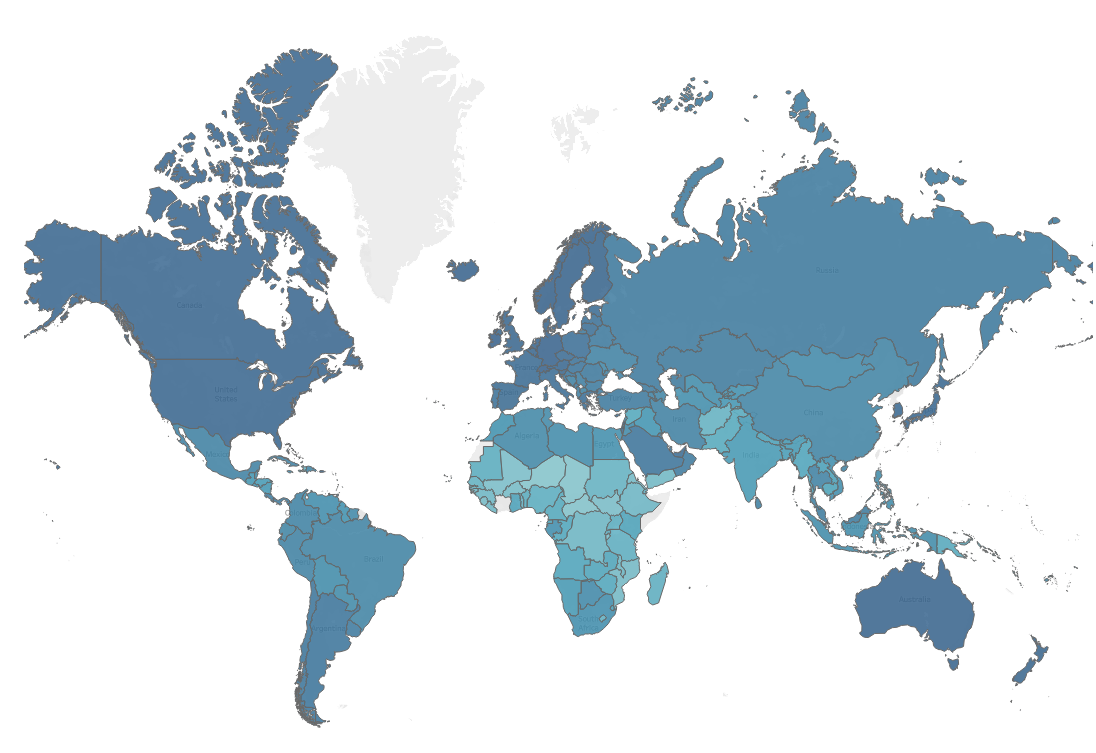
\includegraphics[width=0.5\columnwidth]{wmap.png} 
	\caption{HDI By Country 2019}
	\label{fig1:wmap}
	\end{figure}
\end{center}

The purpose of this visualisation was to get a view of the geographic distribution of HDI (up to 2019, using the HDI dataset), as well as development over time. generally, as expected, Central Africa tends to have lower HDI than the rest of the world. North Africa has seen improvement, with the exception of Libya where HDI decreased drastically during the civil war (and to this day, has not recovered to it's 1990 level). South-East Asia can be seen to have experienced a good deal of gradual, but significant development since 1990. Much of the development in ex-soviet territories can be seen to experience noticeable improvement into the 2000's, where it seems the effects of the de-escalation of cold war tension, and collapse of the USSR had a relatively delayed effect. Generally, countries that had the highest HDI values still showed improvement over the decades. Indeed, there are very few immediately identifiable countries that experienced a regression in HDI. This shows that a quantitative lack of development in countries is not so much their predominant issue, so much as a slow pace. My hypothesis that leads from this, is that negative trends in HDI tend to result from political, civil and/or military conflict, with economic factors completely independent to this and only affecting the rate of development.

\subsubsection*{Factors contributing to HDI}

\begin{figure}[hb]
\centering
\sbox{\measurebox}{%
  \begin{minipage}[b]{.40\textwidth}
  \subfloat
    []
    {\label{fig:figA}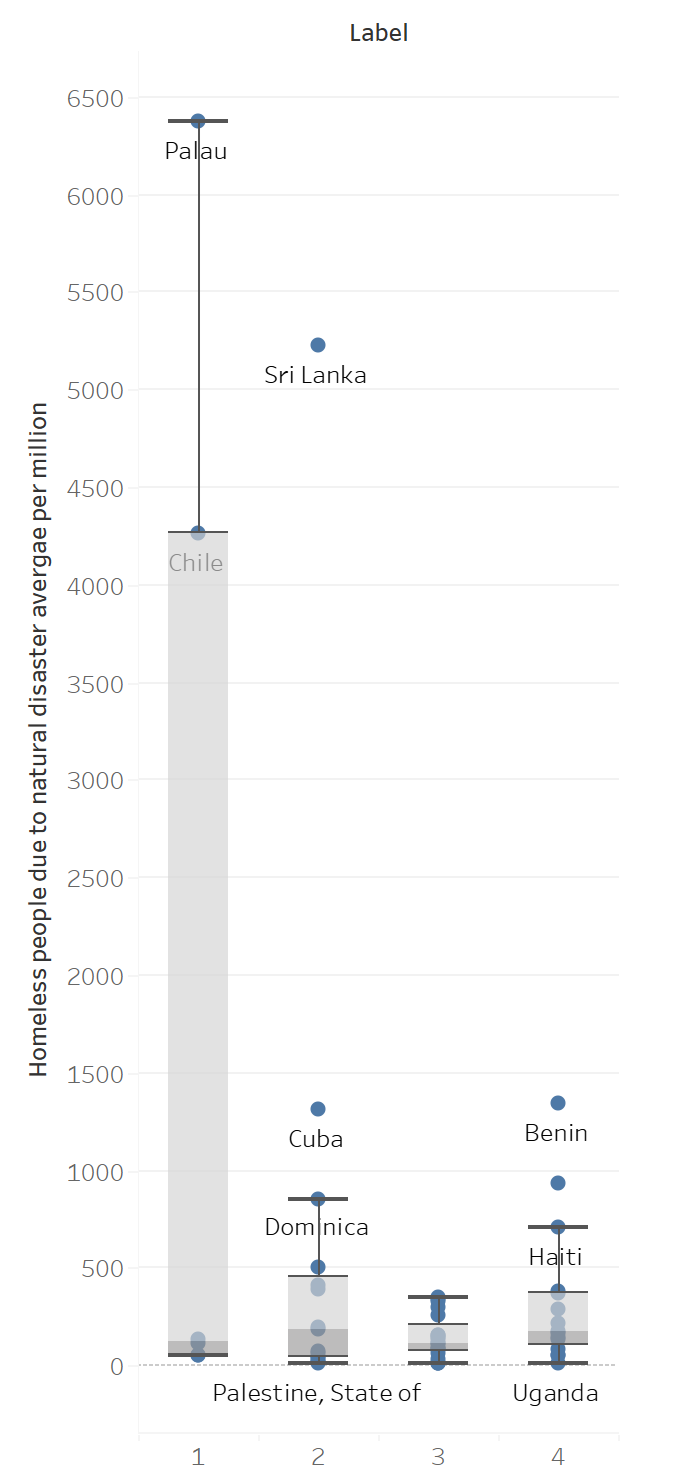
\includegraphics[width=\textwidth,height=15cm]{nat disaster.png}}
  \end{minipage}}
\usebox{\measurebox}\qquad
\begin{minipage}[b][\ht\measurebox][s]{.55\textwidth}
\centering
\subfloat
  []
  {\label{fig:figB}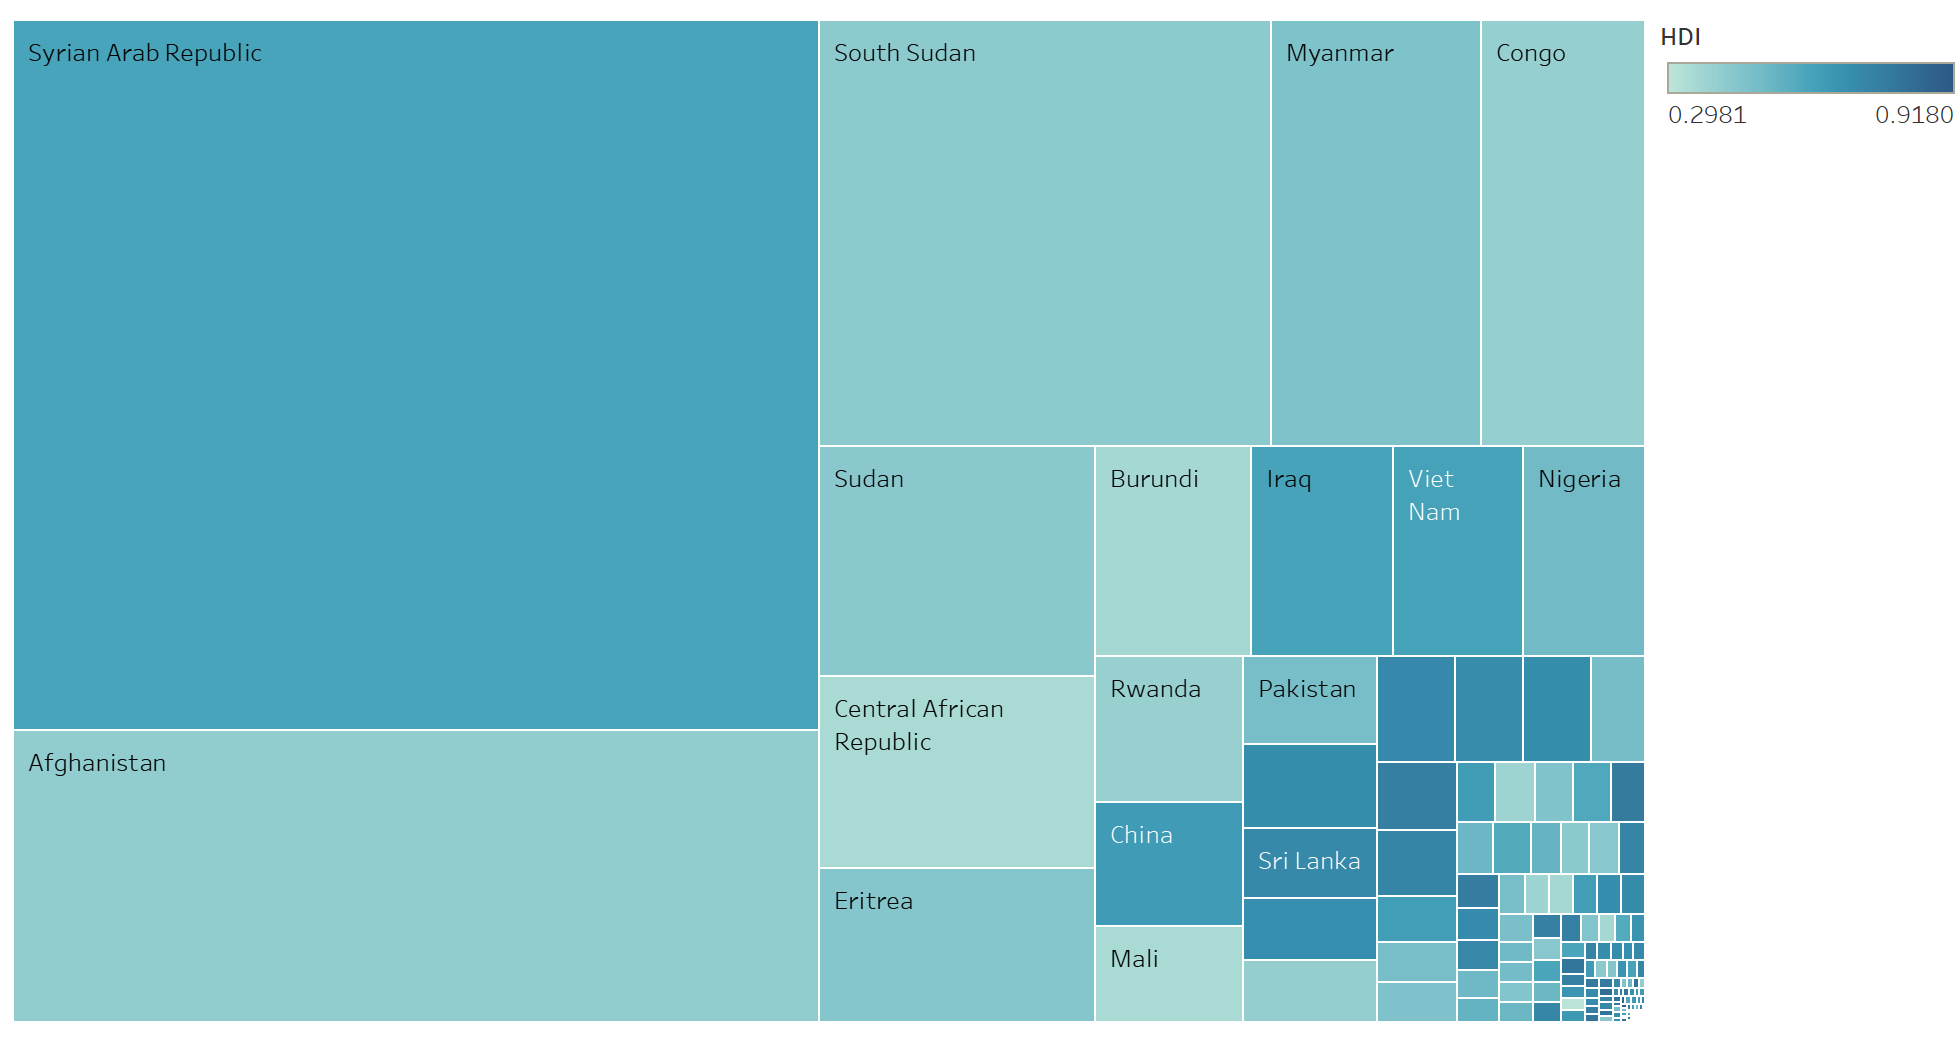
\includegraphics[width=\textwidth,height=7cm]{migration.png}}
\vfill
\subfloat
  []
  {\label{fig:figC}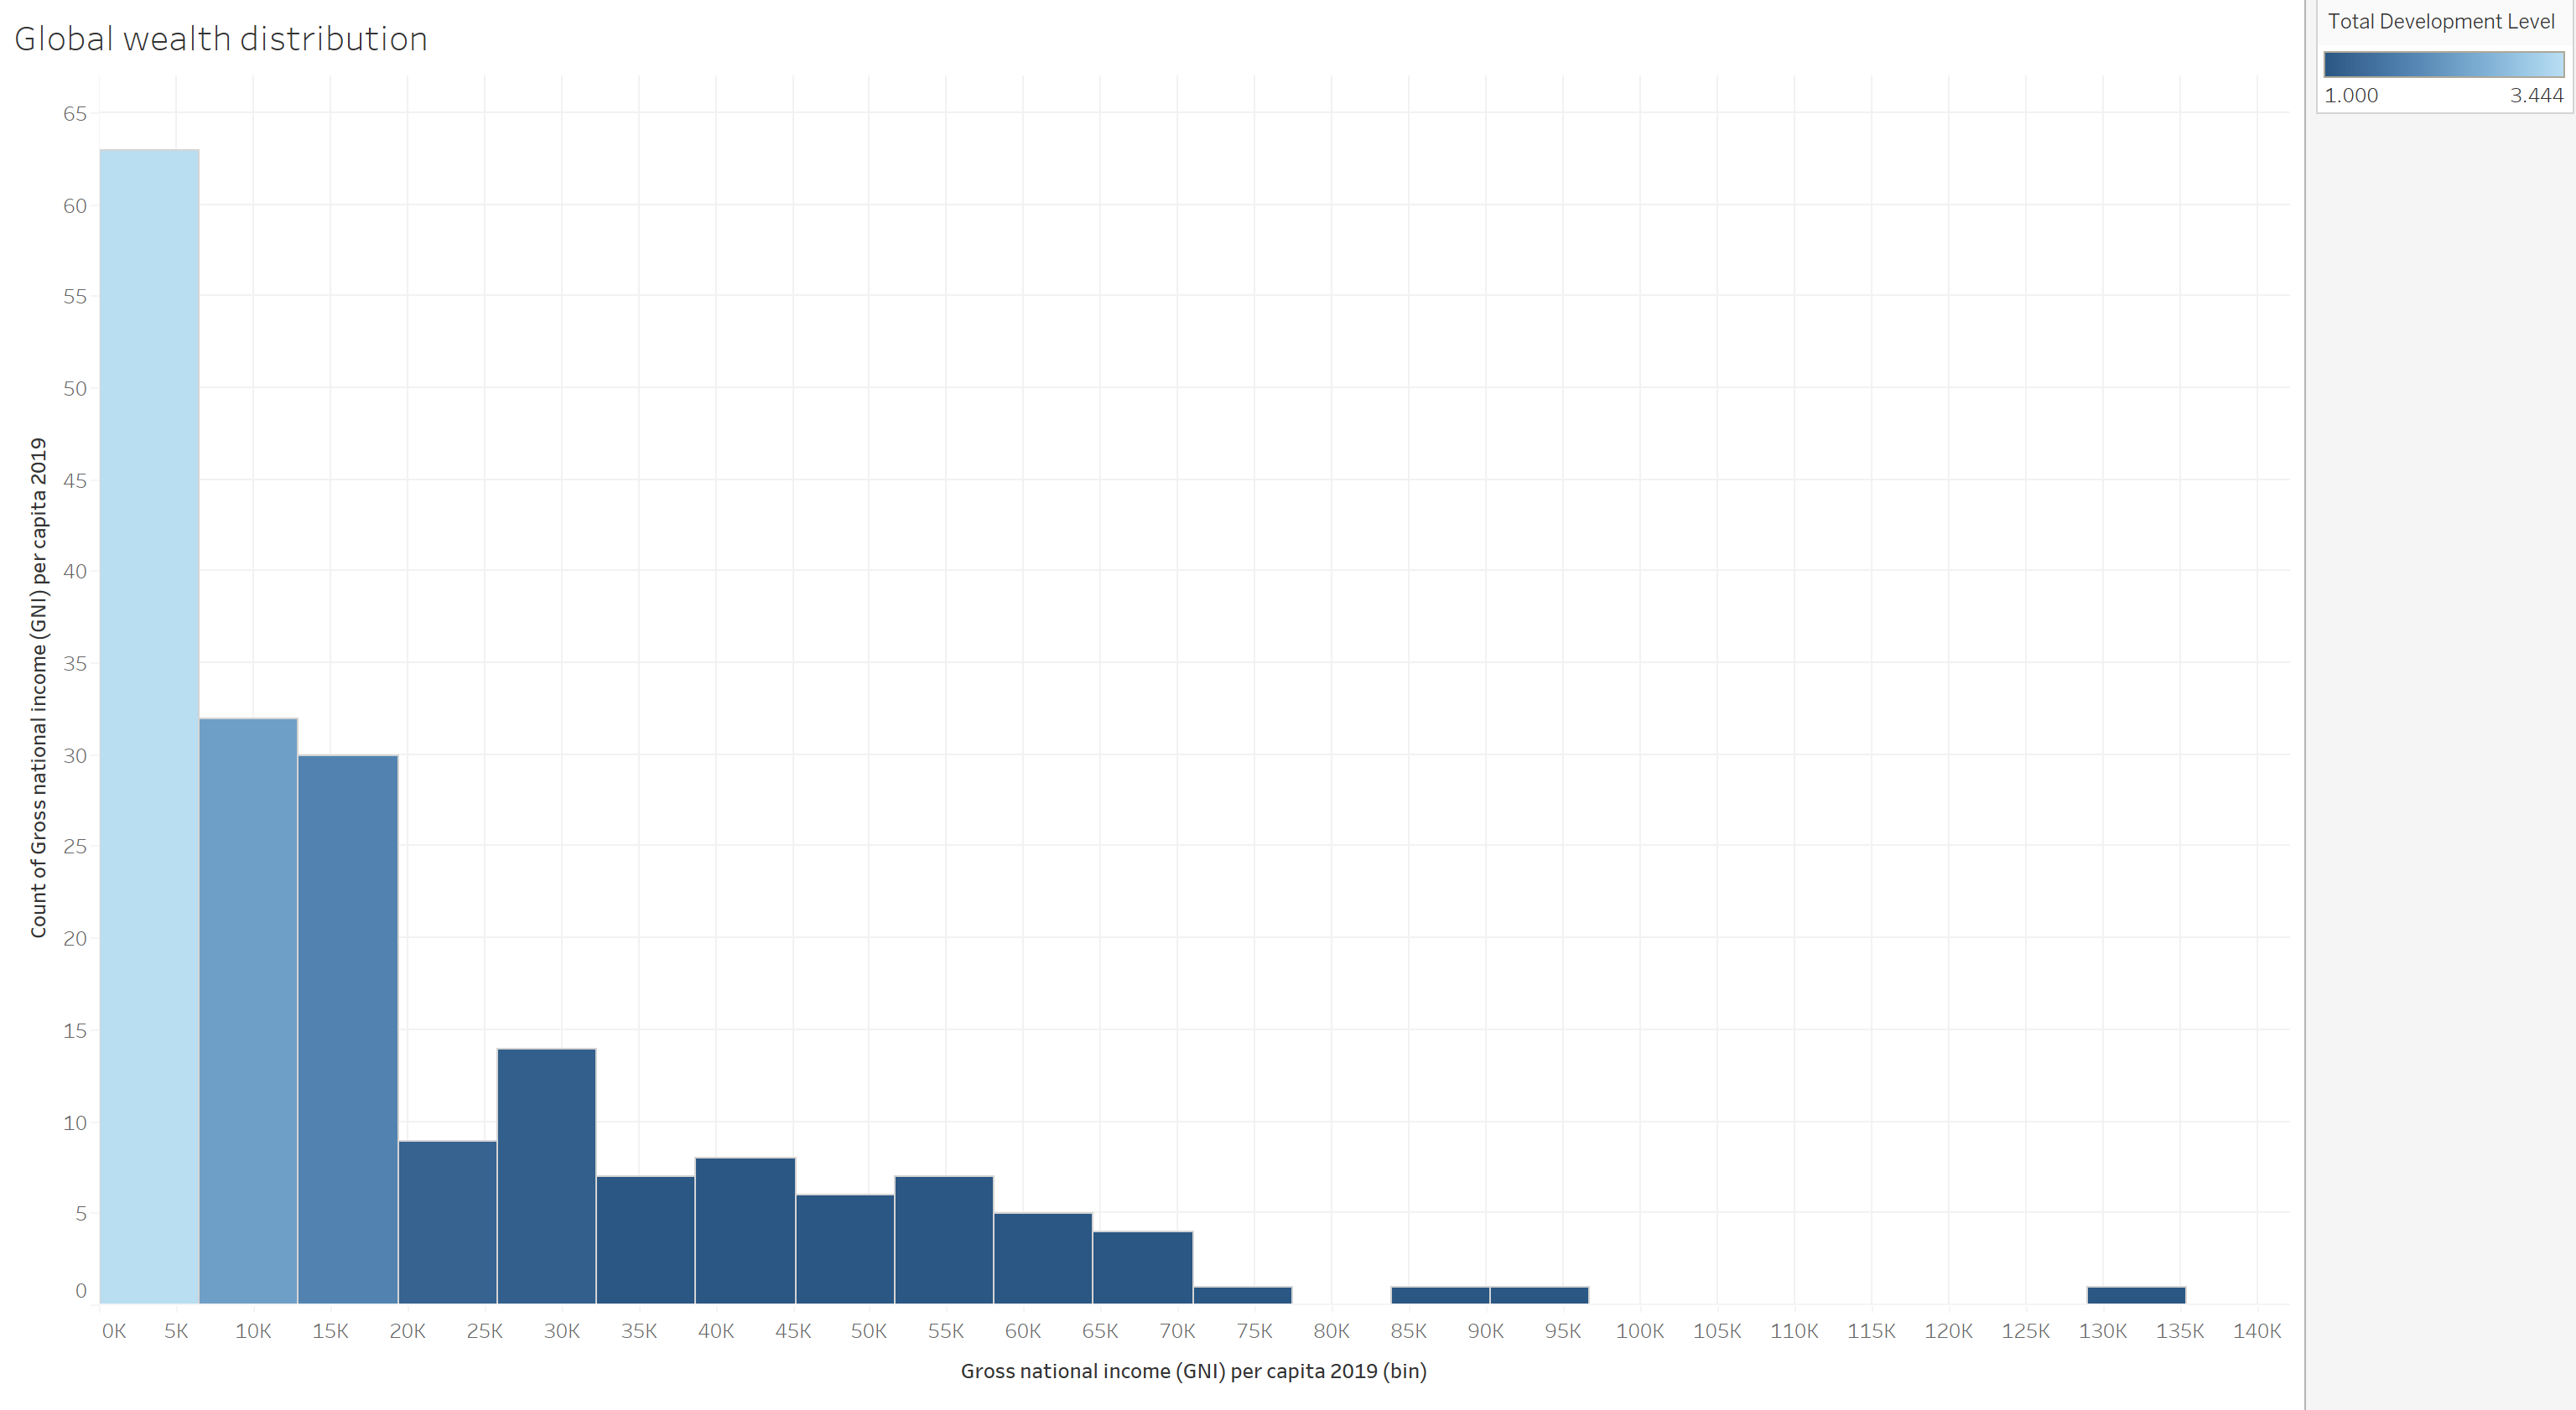
\includegraphics[width=\textwidth,height=7cm]{wealth.png}}
\end{minipage}
\caption{(a) Homelessness due to natural disaster vs development level (b) migration vs HDI by country 2020 (c) distribution of GDP with indications of HDI}
\label{fig:quafdPLOT}
\end{figure}

\clearpage

\begin{center}
\begin{figure}[h!]
    \centering
    \label{fig1:healthED}
	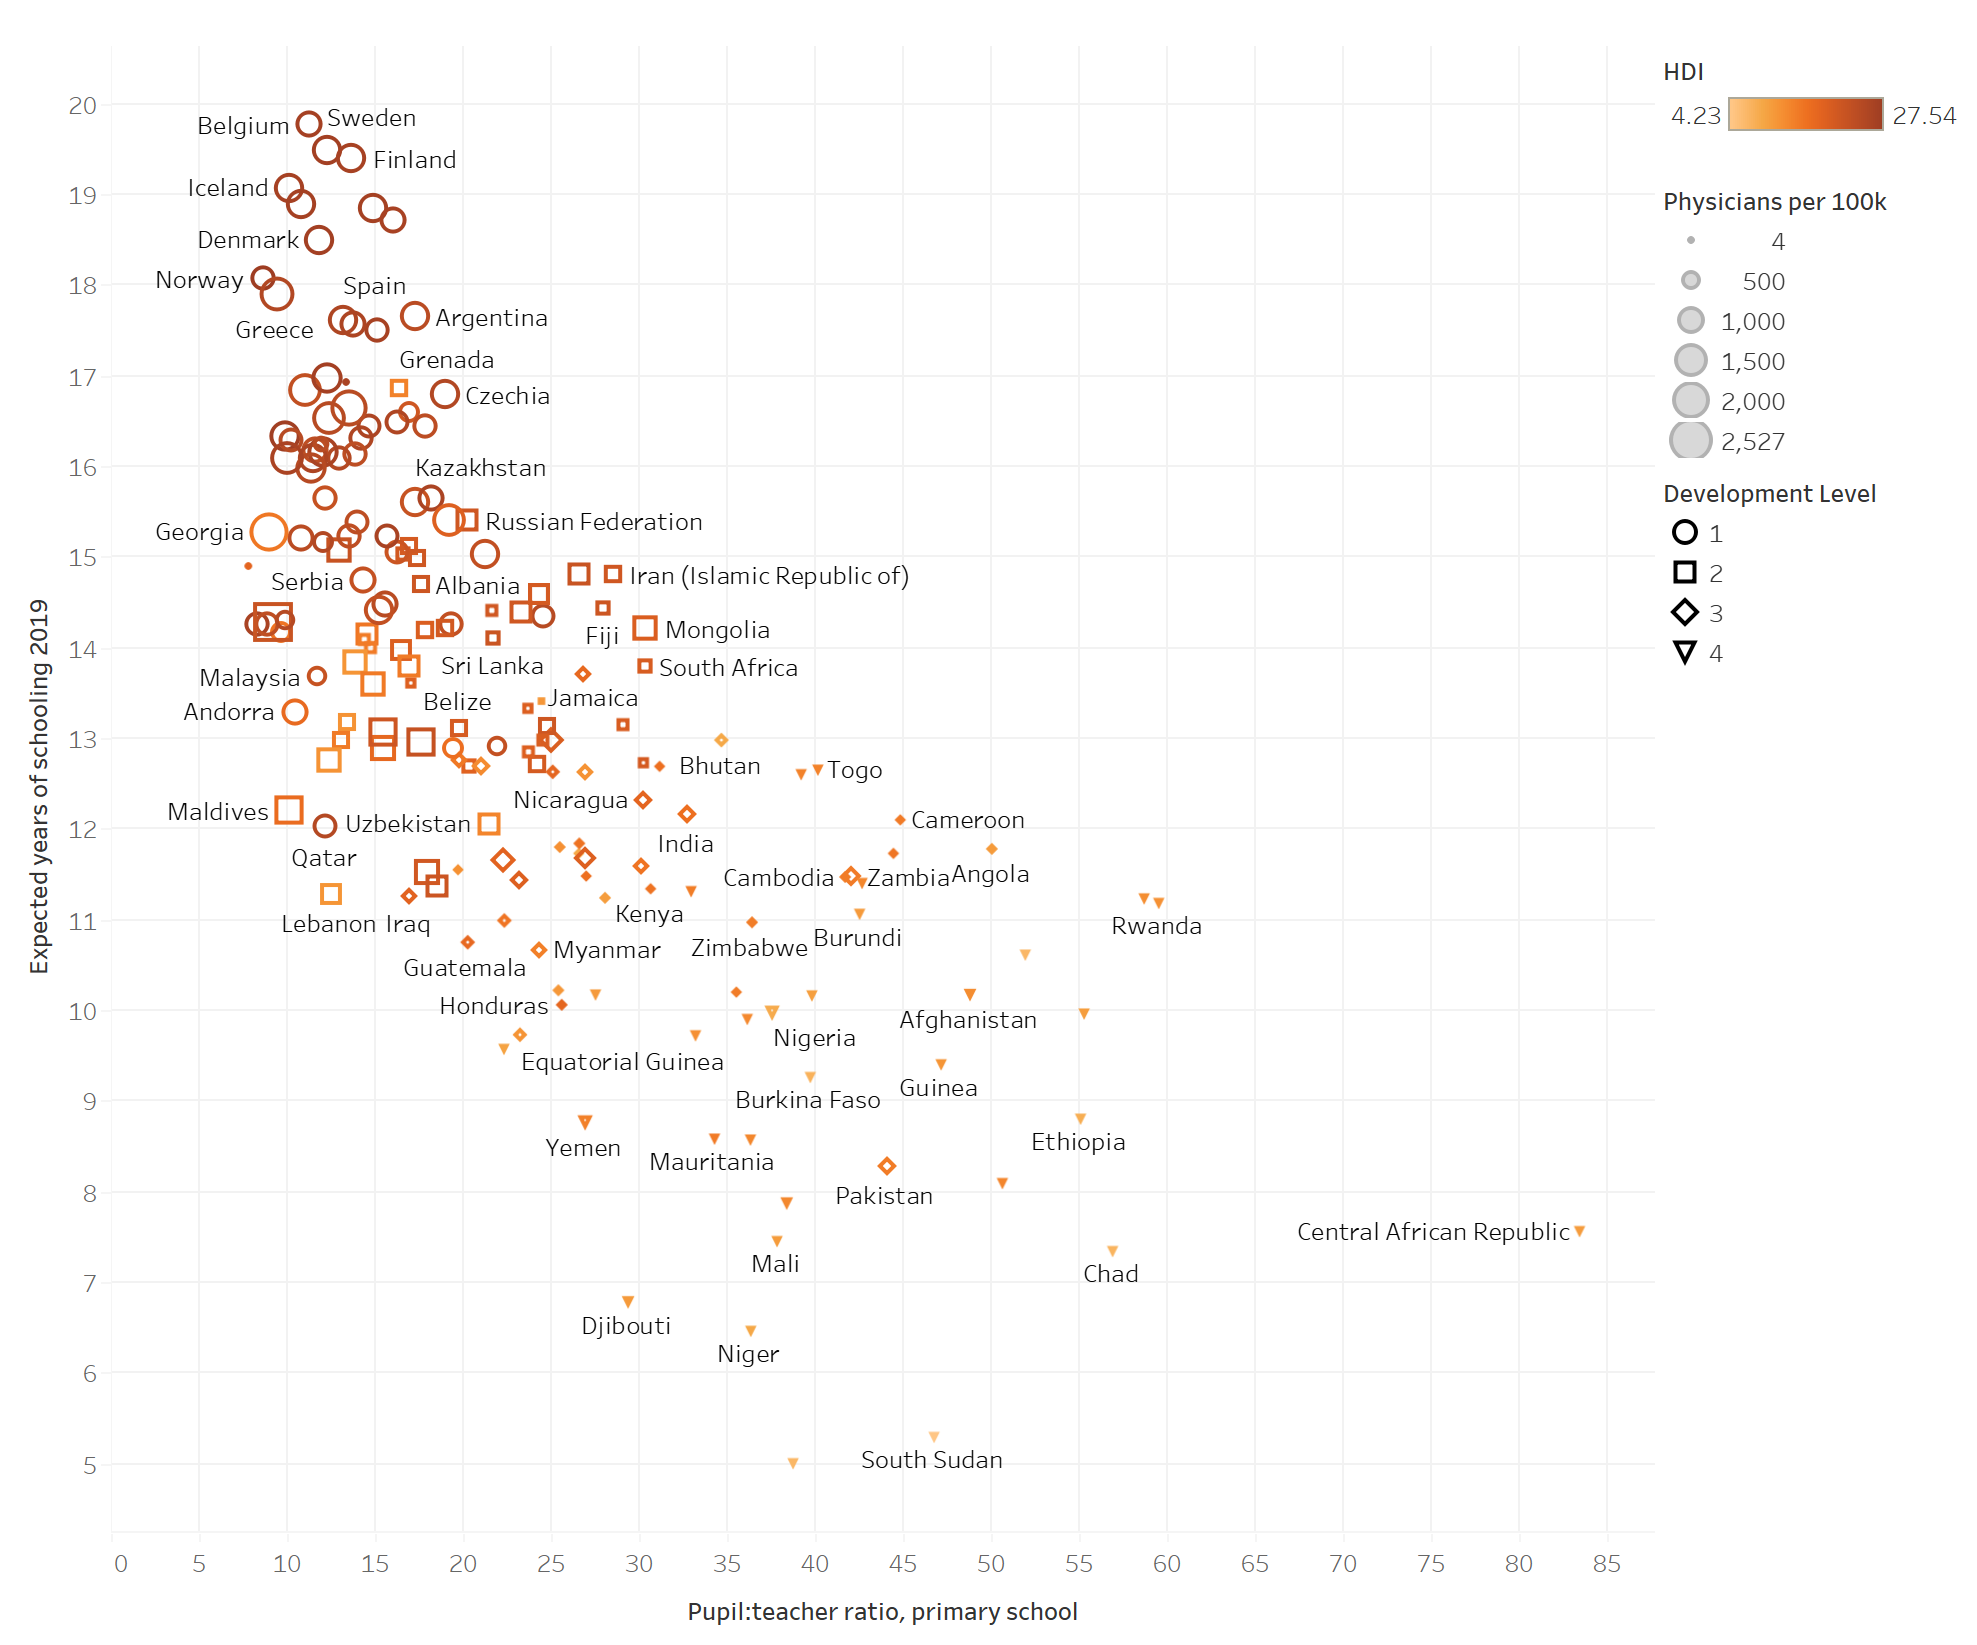
\includegraphics[width=0.75\columnwidth]{healthEducation.png} 
	\caption{Healthcare and Education factors contributing to HDI}
	\end{figure}
\end{center}

The above plots formed my initial foray into exploring the factors that contributing to HDI.

\vspace{0.3cm}

\textbf{Fig 2c: Distribution of wealth.} This plot is clear enough in illustrating economic inequity. With increasing GDP per capita, we see almost exponentially declining numbers of countries that attain this GDP per capita. Note that, with careful inspection of the bars, the 41 countries with GDP per capita over 30k USD are all (or almost all) at Level 1 development. The 23 countries with GDP per capita above 20k are \textit{largely} level 1 also.

\textbf{Fig 2a: Natural disaster homelessness} Based on the initial map, I would expect that countries with large degrees of social upheaval would tend to have lower development levels - there are fewer things that cause more disruption to societies than natural disasters. Plot 2a has some interesting indications. It plots the number of people rendered homeless by natural disaster in each country (normalised per million population), split by level of development. Level 1 development countries have a much lower proportion, with two extreme outliers - Chile and Palau. Both coutries are well known for considerable risk of natural disaster. There may be some trend between levels 2,3, and 4 but if so, this is relatively moderate (albeit more so when the level 1 outliers are excluded from the plot). I would hypothesise as a result, that natural disasters may pose an impact on countries' HDI levels, but rather than being a deciding factor in itself, amplify the effect of existing negative HDI factors. I.e., they have the worst impact when they are placing strain on already under-resourced systems.

\textbf{Fig 2b: Migration} Plot 2b shows the number of refugees by country of origin, with an indication of the HDI of each.Similarly to the distribution of wealth, small numbers of countries have exponentially higher refugee levels . This seems to indicate that refugee crises in a country are relatively rare, but when they occur, they occur in an enormous scale.

\textbf{Fig 3: Healthcare and education} Plot 3 attempts to conglomerate multiple factors, and tries to assess the interplay between them. There are a few trends going on here. The most obvious is that countries with higher average pupil-teacher ratios have far fewer expected years of schooling for students born in 2019.

Further, countries with more doctors per 100k population have much higher HDI - this also correlates to expected years of education. This does lead to the rather obvious hypothesis that with longer education, and smaller class sizes, leads to a positive feedback loop in societies - more education means more qualified doctors and teachers, which leads to more young people living longer and healthier, and getting more education. Tying it back into the plots above, I would hypothesise that a somewhat under-appreciated consequence of war, civil unrest etc, (apart from the obvious horrors of widespread death, disarray and destruction) is the debilitating impact it has on education where they take place.


\subsection*{Specific Observations} 

\textbf{ORDERING BY COUNTRY} 

\vspace{1cm}

\hfill \break  

\begin{figure}[hb]
    \centering
    \subfloat[\centering Noticeable decline in HDI in Syria at the outbreak of civil war]{{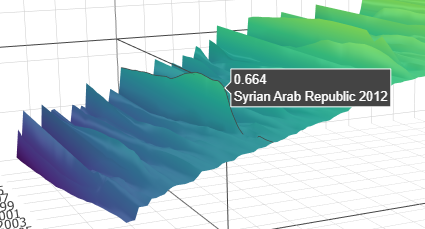
\includegraphics[width=0.45\columnwidth]{syria.png} }}%
    \qquad
    \subfloat[\centering Noticeable uptick in HDI in Rwanda following the end of the civil war.]{{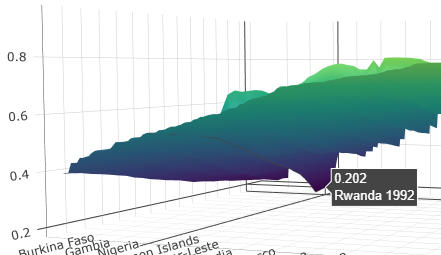
\includegraphics[width=0.45\columnwidth]{rwanda.png} }}%
    \caption{Small extracts from the HDI time series surface plot}%
    \label{fig:surfaceplot}
\end{figure}

\textbf{Fig 4. Ordering Countries by HDI over time} 

\vspace{0.25cm}

Based on Figure 1, I thought it would be interesting to delve into more detail as to how HDI ratings have developed over time. The animated map, while very effective at illustrating the geographic distribution of HDI, made it difficult to identify unexpected individual behaviours \textit{over time}. I plotted a 3d surface using the plotly library in R. This plots HDI by country and year, which allowed me to identify interesting behaviours over time much more easily and flexibly, compared to constantly iterating through the frames of the animation of Figure 1. Note that 3d plots are only really useful and effective when used in an interactive manner - a 3d surface cannot be completely communicated in a single 2d image. A link to the interactive plot is here\footnote{https://andrew-nash.github.io/p1.1.html} (page may take a few seconds to load) - I encourage the reader to take some time to interact with this plot.

Figures 4a and 4b show two (of many, many possible) insights that were immediately obvious upon first inspection. Syria can be seen to take a massive downturn in terms of its HDI at 2012 - un-coincidentally, a year after the beginning of the Syrian civil war. On the flipside, Rwanda can be seen to take a massive uptick in HDI around 1992 - the year a ceasefire was declared in the civil war at the time. 

This seems to reinforce general observations from above - civil unrest is the worst cause of detriment to the HDI ranking (and by assumption, the quality of life in a country), and is the main cause for any country to regress in terms of HDI.


\hfill \break  

\begin{figure}[H]
    \centering
    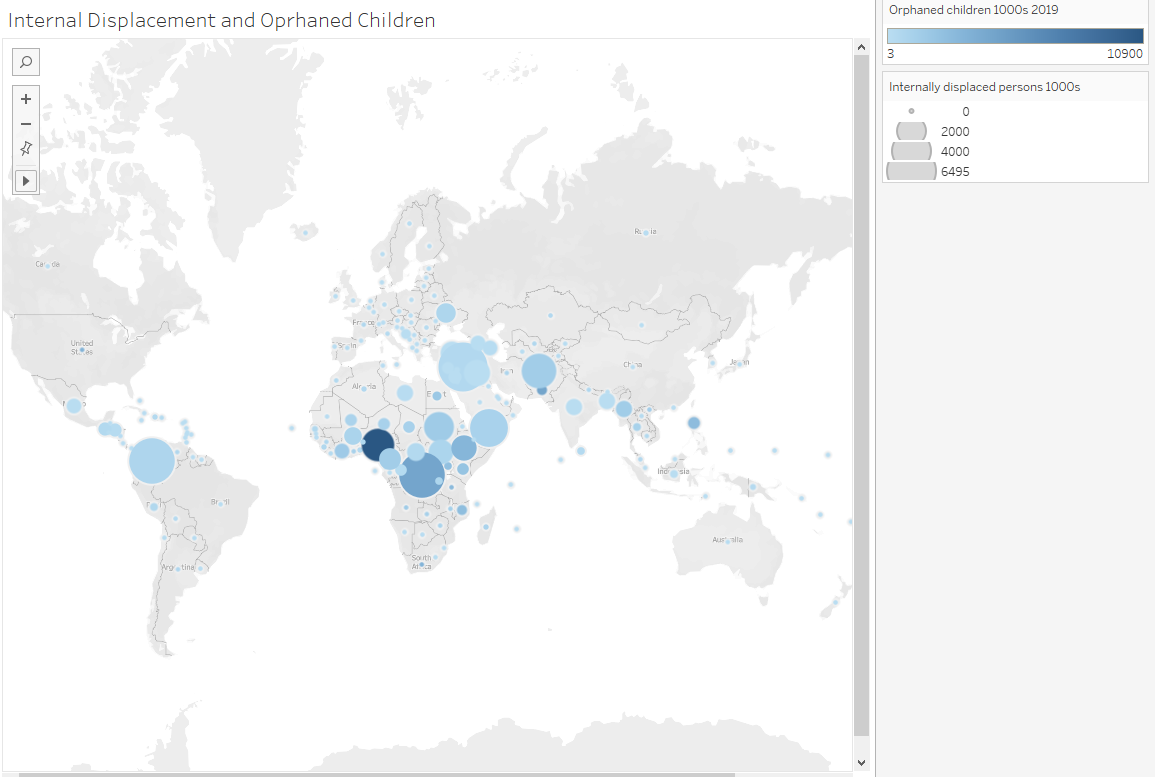
\includegraphics[width=\columnwidth]{orphans.PNG} 
    \caption{Comparing rates of internal displacement, and amounts of orphans by country}
    \label{fig:orphans}
\end{figure}

\textbf{Fig \ref{fig:orphans}. Ordering countries by internally displaced persons, and oprhans} 

\vspace{0.25cm}

In figure \ref{fig:orphans}, I considered the distribution of internally displaced persons, and orphans, by country. There is an obvious correlation between the two - the few countries with high quantities of internally displaced persons also tend to see large amounts of orphans (both stemming from common issues of war and strife). In terms of spurious values, there are an obvious few. As we've previously seen, Syria has a high amount of internally displaced persons (correlating to its high amount of egressing refugees), as does the Congo. Even more tragically, however, is the phenomenal quantity of orphaned children in Nigeria - what appears to the on the order of 10M. This is unexpectedly far higher than any reasonable expectation, looking at the values of all other countries worldwide.


\textbf{IDENTIFYING CORRELATIONS} 

\vspace{1cm}



\begin{center}
\begin{figure}[H]
    \centering
	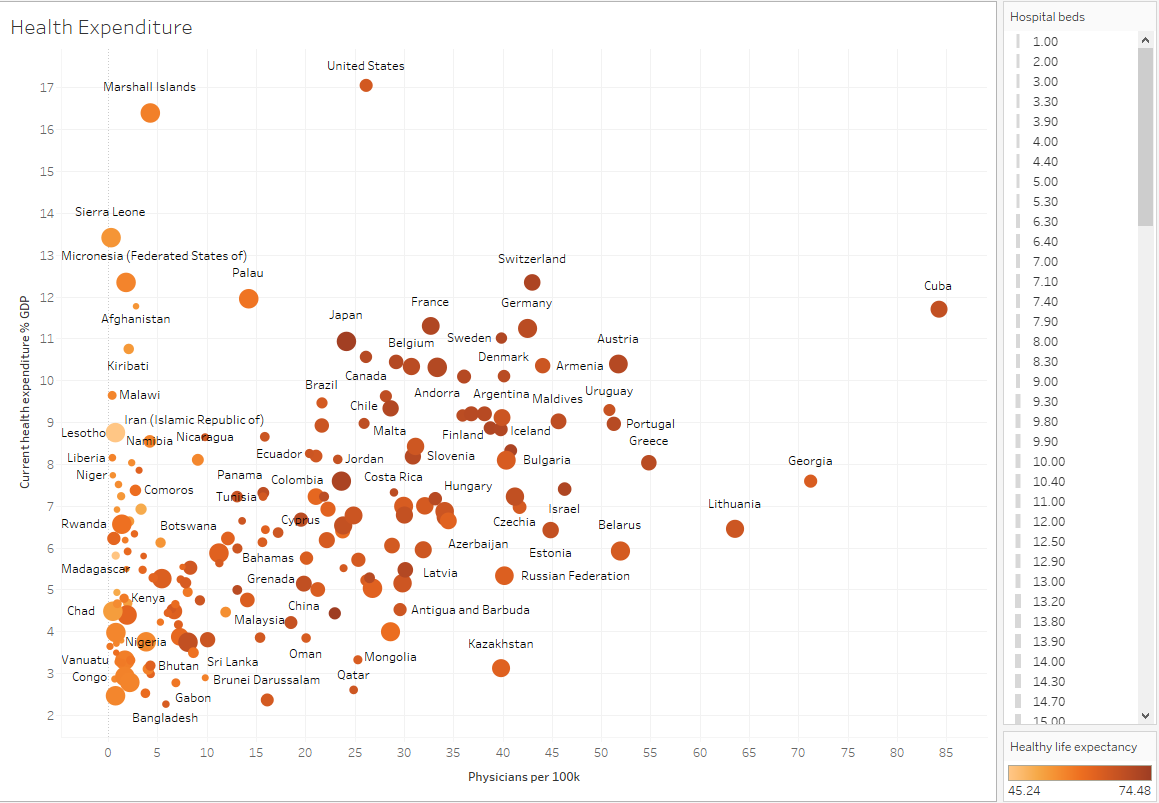
\includegraphics[width=0.75\columnwidth]{healthcareObs.PNG} 
	\caption{A deep dive on healthcare and life expectancy}
	\label{fig:healthcare}
	\end{figure}
\end{center}

\textbf{Fig \ref{fig:healthcare}. Healthcare expenditure} 

\vspace{0.25cm}

There is a joint correlation between expenditure on healthcare, physicians per 100k and available hospital beds with life expectancy. As an obvious correlation, countries that spend a higher percentage of their GDP tend to have a higher proportion of doctors. Interestingly, the same is not seemingly true of the proportion of healthcare spending to hospital beds. Life expectancy also (obviously) tends to be higher with higher numbers of physicians per 100000, but the same isn't strictly true with health expenditure.

The United States is a notable outlier here, with stratospheric healthcare spending, yet surprisingly low numbers of physicians, beds and life expectancy.

\begin{center}
\begin{figure}[H]
    \centering
	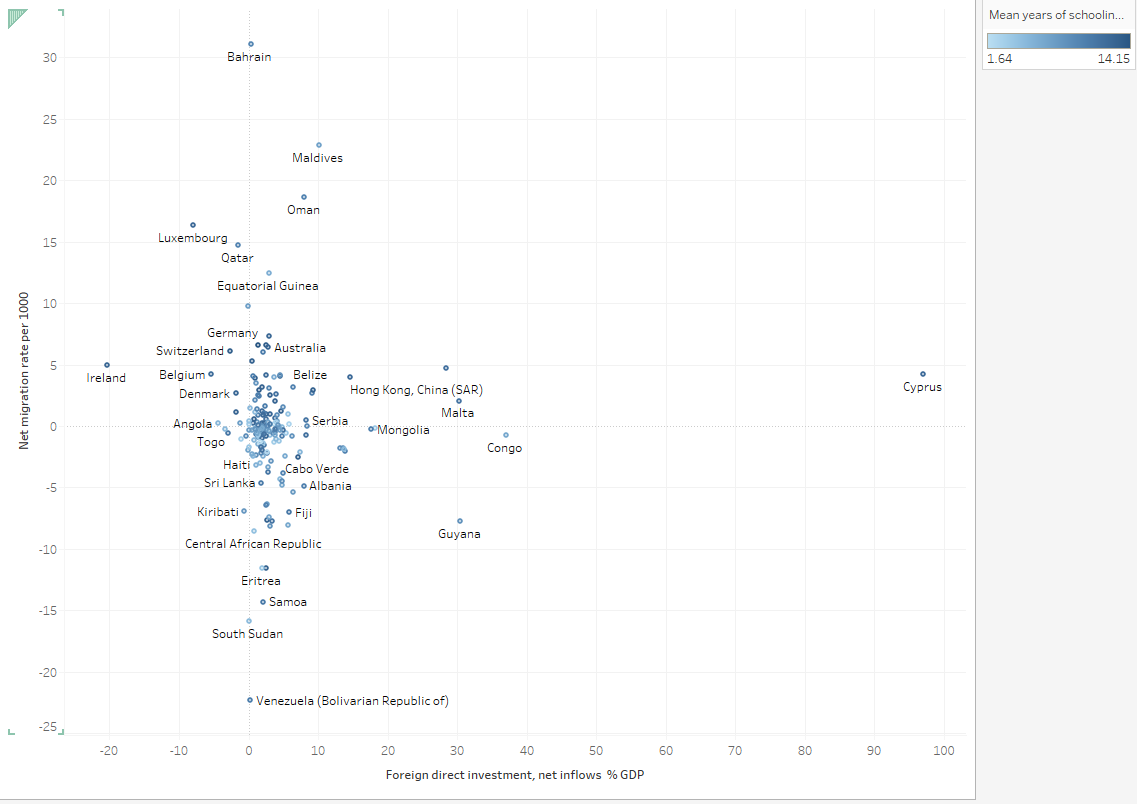
\includegraphics[width=0.75\columnwidth]{fdi.PNG} 
	\caption{Looking at foreign investment}
	\label{fig:fdi}
	\end{figure}
\end{center}

\textbf{Fig \ref{fig:fdi}. Foreign investment} 

\vspace{0.25cm}

Very surprisingly, when plotting FDI against migration, there is no correlation of any sort.  Incorporating mean years of education leads to no noticeable correlation either. This is quite a surprise, as I'd expect lack of economic opportunities (particularly from foreign multinationals) would lead to large amounts of emigration.

An interesting outlier here is Ireland - with a quoted FDI of -20\% of our GDP, we seem to have the lowest in the world. I validated this in the original dataset, it is not a mistake, or a corruption, but the value that the UN quote in the report. I can only assume this anomaly is a result of our corporate taxation system that has generated international controversy recently. 

\begin{center}
\begin{figure}[H]
    \centering
    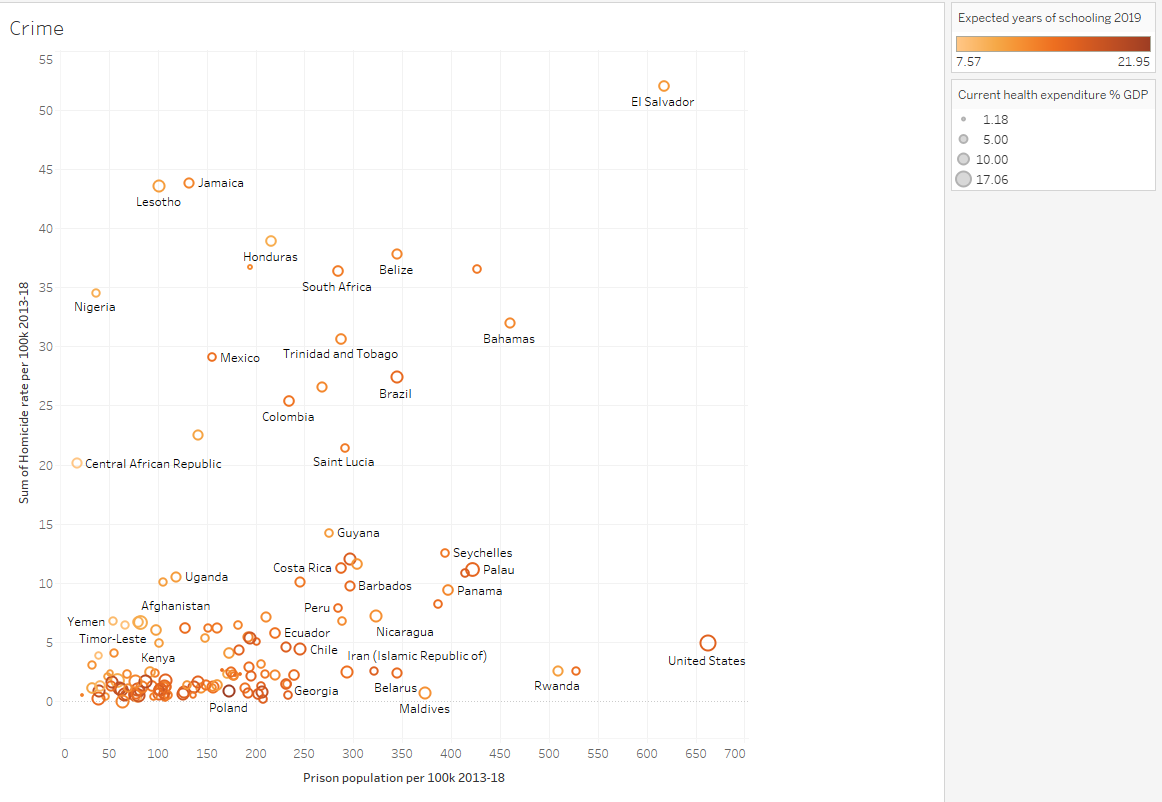
\includegraphics[width=0.75\columnwidth]{crime.PNG} 
	\caption{Crime}
	\label{fig:crime}
	\end{figure}
\end{center}

\textbf{Fig \ref{fig:crime}. Crime} 

\vspace{0.25cm}

In general, this plot seems to indicate that there is not a significant correlation between the number of homicides in a country, and the prison population. It does seem, however, that countries with higher mean years of education have lower prison populations, but this is not certain. This is, naturally quite a surprise, since you would expect homicide rates to act as a general indicator of crime rates, which should in theory correlate to prison populations.

\begin{center}
\begin{figure}[H]
    \centering
	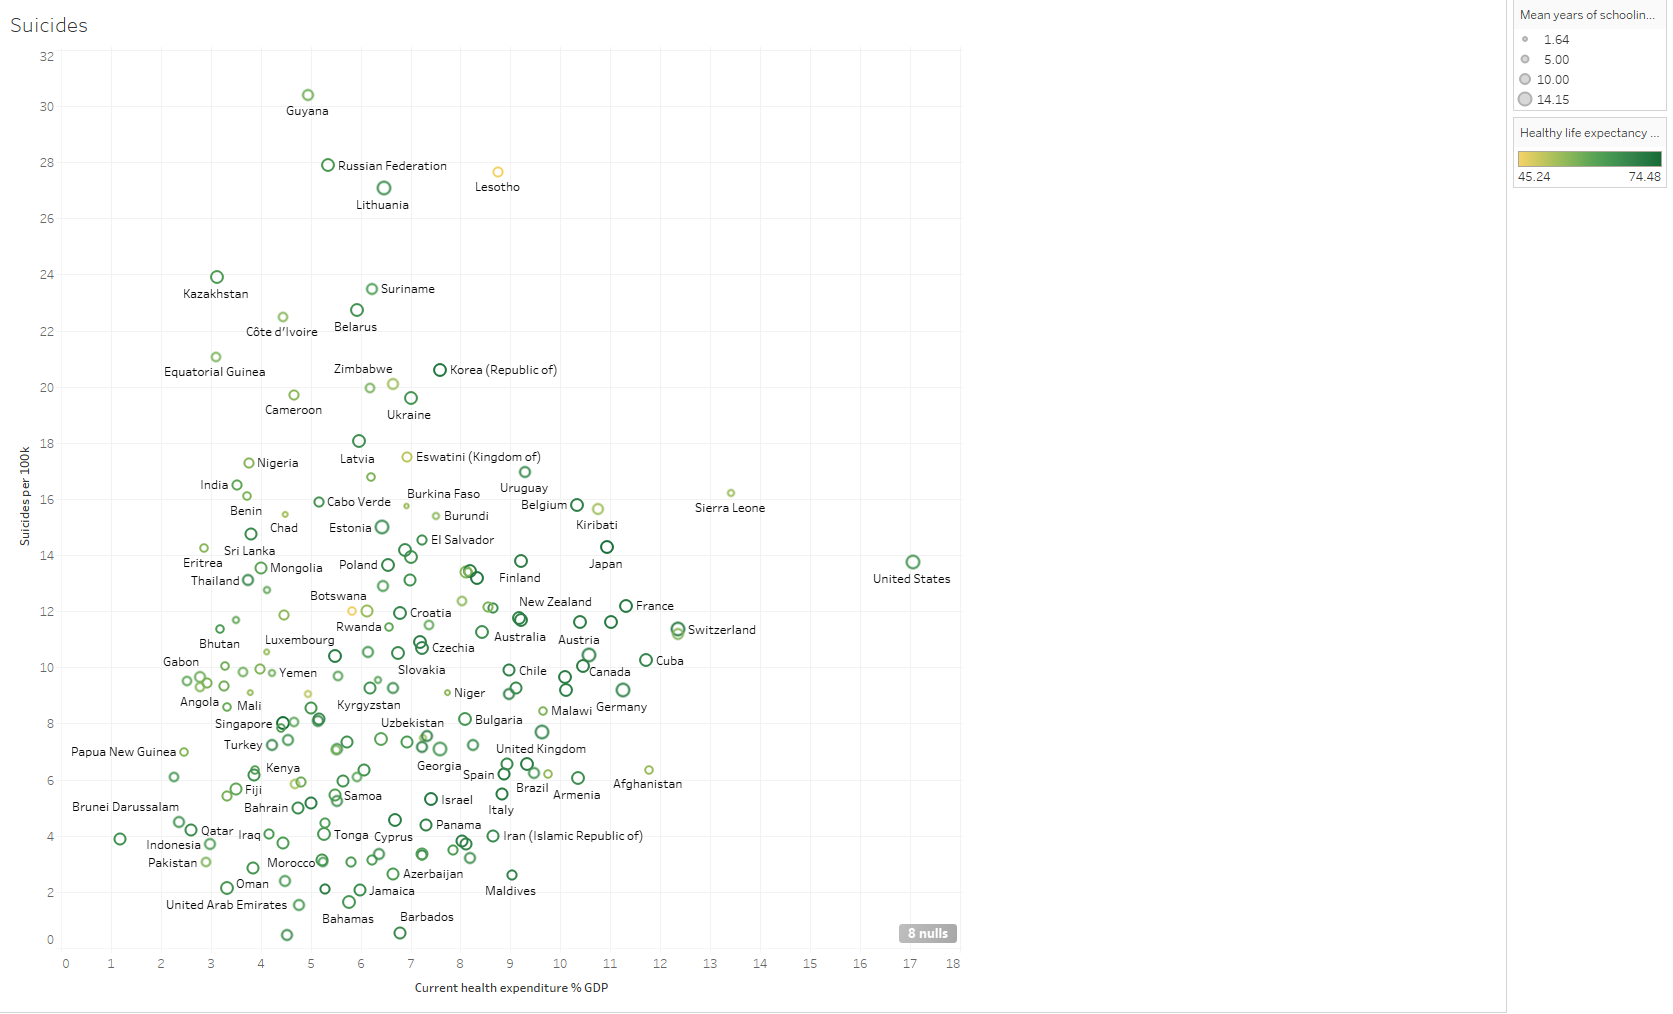
\includegraphics[width=0.75\columnwidth]{suicides.PNG} 
	\caption{Suicide rates}
	\label{fig:suicide}
	\end{figure}
\end{center}

\textbf{Fig \ref{fig:suicide}. Suicide rates} 

\vspace{0.25cm}
This plot shows that there is a quite weak, but non-negligible correlation, surprisingly, between the health expenditure of a country, and its suicide rate. An important fact of note here is that this may be a result of reporting differences, rather than differences in the true underlying phenomena. 

\vspace{0.8cm}

\textbf{PATTERNS AND HYPOTHESIS} 

\vspace{0.8cm}

\textit{Hypothesis 1: War is main factor impacting the development level of a country}
Referring to Figures \ref{fig:surfaceplot} and \ref{fig:quafdPLOT}, we see the lowest development levels, and the greatest changes in HDI, in countries experiencing war and civil wars. We see through homelessness from natural disasters that these catastrophic, natural events alone are not necessarily a guarantee of a low level of development, in any way close to the same manner as wars do. The hypothesis leading from this is that wars, civil wars, and large scale civil unrest are the single most detrimental factors to the standard of living in a country. As an aside, this is another reason that the current invasion of Ukraine is all the more disheartening and tragic.

\textit{Hypothesis 2: healthcare has large fixed cost}
Referring to Figure \ref{fig:healthcare}, we see that, amongst other things, the percentage of GDP spent on healthacre does not completely guarantee higher life expectancies. We see a correlation from this spend to the number of physicians per 100k, and from this number of physicians to the life expectancy - but I hypothesise that the correlation between spending and life expectancy is transitive through the amount of doctors and beds rather than direct. This means that, for countries with low GDP, they must spend a much higher proportion of their total GDP to reach the level of doctors and facilities. Put simply, I hypothesise that poorer countries (in terms of GDP per capita), have to spend more money, relatively to high GDP per capita countries, in order to attain a higher life expectancy.

\textit{Hypothesis 3: mass migration is driven far more by social rather than economic reasons}
This leads on from hypothesis 1, and is reinforced by the fact that foreign investment does not seem to drive investment. A possible alternative possibility, is that a lack of domestic industry is more important in driving emigration than a lack of foreign investment. Overall, I'd expect that improving the social conditions internal to a country, from within that country (as compared to by intervention of foreign companies), are much more important in preventing mass emigration.  This is quite counter-intuitive, as before the assignment, I'd have expected the reverse to be true.

\textit{Hypothesis 4: countries with higher prison populations do not necessarily have higher crime rates}
Referring to Figure \ref{fig:crime}, my hypothesis here is simple - the main factor influencing the prison population of a country is not the rate at which crimes are committed, but the political/legal decisions as to the severity of that crime in the country. Put simply, it is the extent of punishment that drives the prison population figures, rather than the criminality in a country. 

\textit{Hypothesis 5: more developed countries may potentially have higher suicide rates}
This is somewhat more speculative. My hypothesis, looking at Figure \ref{fig:suicide}, is that more developed countries experience higher rates of death by suicide than less developed countries. The alternative hypothesis would be that any difference is due to the fact that countries with better healthcare systems monitor the figures for causes of deaths more effectively, leading to this discrepancy. Since the alternative hypothesis calls into question the integrity of the data, we cannot test it with the HDR dataset, but with more information, it would be very interesting to assess.


\vspace{0.8cm}

\textbf{UTILITY OF DIFFERENT VISUALISATIONS} 

\vspace{0.8cm}

The first obvious comparison to draw is between the first Figure in the document, the map in Figure \ref{fig1:wmap}, to the surface plot in Figure \ref{fig:surfaceplot}. These both visualise the same data, but in very different ways. Effectively, the difference is that the animated map shows the data with 2 space and 1 time dimensions, whereas the surface plot conveys the same information in 3 space dimensions. The 3 space dimensions are vastly superior, for the simple reason that it is much easier to internalise the information at your own place. With the 2+1 plot, you can only look at the map at one point in time, at one moment in time, and you therefore rely on memory and perception to notice changes over time. For the surface plot, you can viscerally perceive those changes over time, all at the same time. An important drawback however, is that any 3d plot must be interactive to be effective - when constrained to a 2d projection of the surface, you cannot ever get a full understanding of the different behaviours in the plot. For instance, the changes for Libya are hard to notice in the animated map, and the jump in Rwanda at 1998 is very hard to spot, unless you are interacting with the plot, and happen to rotate into the correct position.


Consider the box-and whisker plot int Figure \ref{fig:quafdPLOT}. This plot indicates no real correlation between homelessness due to natural disaster, and development level. This visualisation has two flaws that I thought would be interesting to attempt to correct. First, it is very sensitive to outliers, which obscure trend, and gives no sense of regionality or location - of particular import when natural disasters are a very location-dependant phenomenon. The natural next step is therefore to try to incorporate this onto a map. 

\begin{center}
\begin{figure}[H]
    \centering
	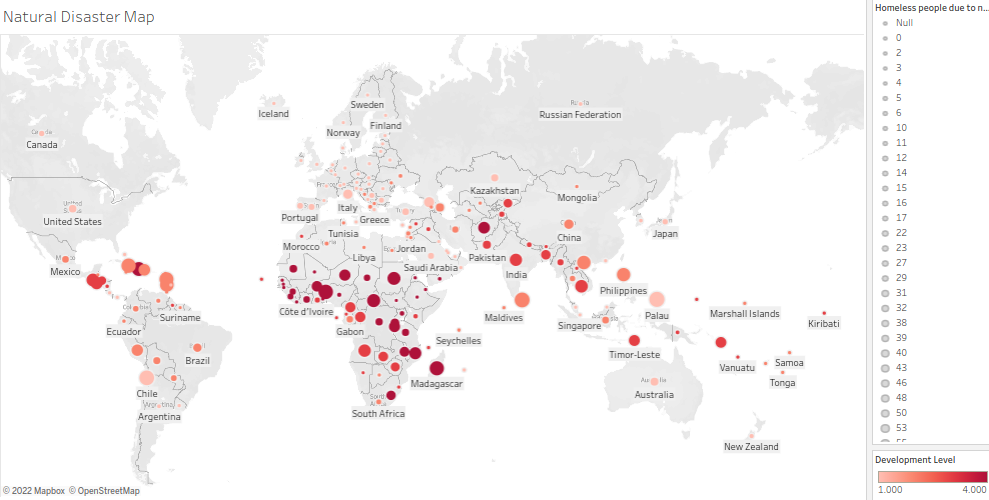
\includegraphics[width=0.75\columnwidth]{natDISMAP.png} 
	\caption{Natural disaster homelessness by development level}
	\label{fig:disastermap}
	\end{figure}
\end{center}

This is clearly much better, and goes some way to contradicting the initial hypothesis taken in part from the box-and whisker plot - we see that countries with high natural disaster homelessness are likely to be development level 4 countries in Africa, with a tendency for them to be 2 and 3 in Cental and South America and South East Asia. The plot has the disadvantage of the sizes of the circles being harder to  compare, than positions of points in the box and whisker, but in this case, the interpretability advantages far outweigh this.


\vspace{2.0cm}


\section*{Task 2 \\ Multidimensional Projections}

The classes and their colourings are as follows:\\
Buses - greeny teal \\ 
African tribes - blue \\
Elephants - green \\ 
Buildings - bluey teal \\
Horses - yellow \\ 
Food - red \\
Beaches - blue \\ 
Mountains - orange\\
Flowers - greenish yellow\\
Dinosaurs - green

\subsubsection*{Part A - exploring an image collection}

\subsubsection*{Neighbour Joining Tree}
\begin{center}
\begin{figure}[H]
    \centering
	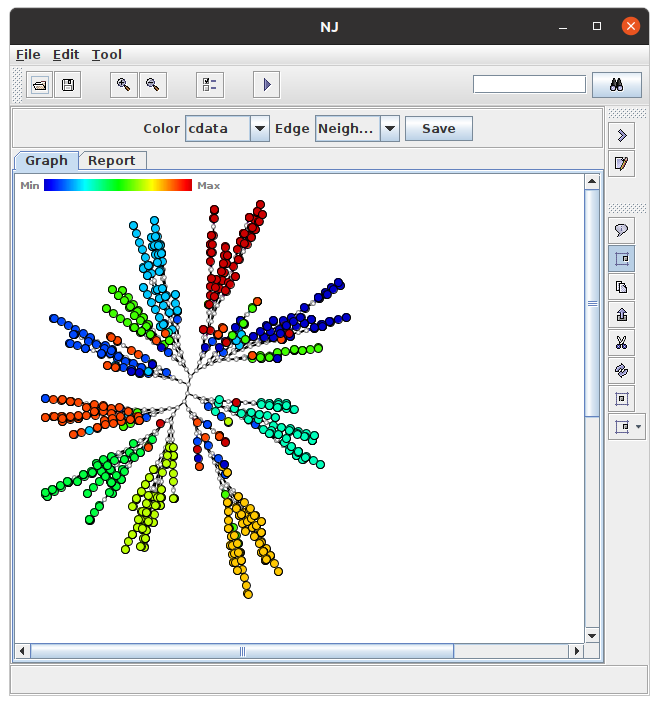
\includegraphics[width=0.75\columnwidth]{neighbourJoining.png} 
	\caption{Neighbour Joining}
	\label{fig:nj}
	\end{figure}
\end{center}

For a relatively simple algorithm, this has led to a surpisingly good results - the branches of the tree are quite homogenous. Some classes are almost perfectly segemented, namely dinosaurs, flowers, and food. 

When looking at the misplaced images, some interesting observations can be made. The predominant overlap occurs where images feature very similar colour palettes. E.g., certain images of African Tribes feature vibrant contrasting colours, that occur in similar proportion in some exotic food dishes. Further, African Tribes are often pictured in desert landscapes that bear some resemblance to beaches. Elpehants, as a large grey mass are in that sense similar to mountains. THis accounts for the majority of the overlap. 

An interesting example can be seen below, where the elephants are very much of the same colour of the mountains in neighbouring images, but also the shape of the clouds in the background are very similar to those of a mountain.

\begin{center}
\begin{figure}[H]
    \centering
	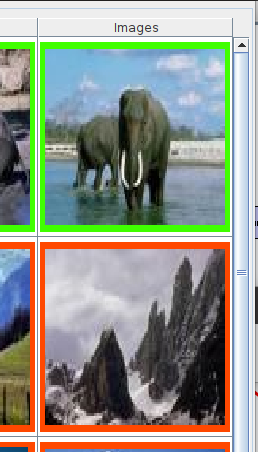
\includegraphics[width=0.5\columnwidth]{elephant and mountain.png} 
	\caption{Example of confused images}
	\label{fig:elephantMt}
	\end{figure}
\end{center}

A more general perspective shows how colour is a key factor in determining similarity

\begin{center}
\begin{figure}[H]
    \centering
	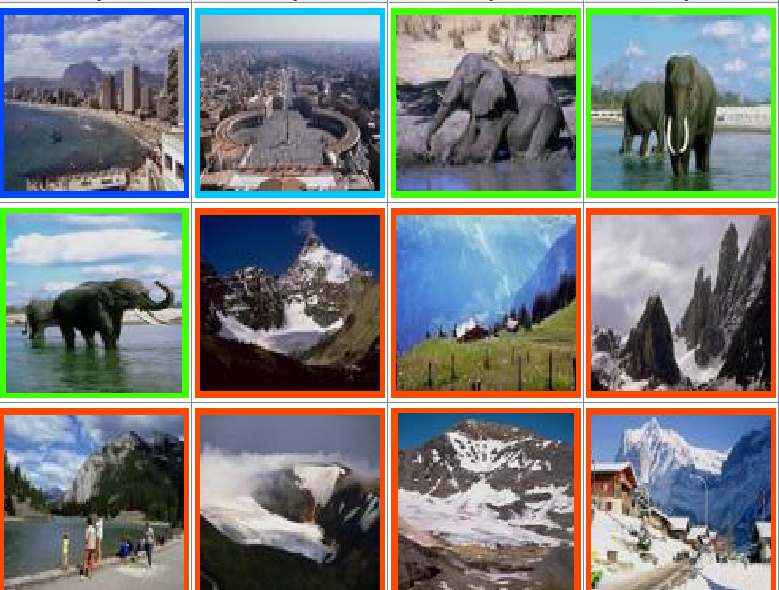
\includegraphics[width=0.75\columnwidth]{greys.png} 
	\caption{Even though the contents of these images are very different, and although they correspond to different classes, they contain the same colours in similar proportions.}
	\label{fig:greys}
	\end{figure}
\end{center}
\subsubsection*{LSP} 

\vspace{0.5cm}

\begin{figure}[H]
\centering
\sbox{\measurebox}{%
  \begin{minipage}[b]{.40\textwidth}
  \subfloat
  []
  {\label{fig:lsp10Panel}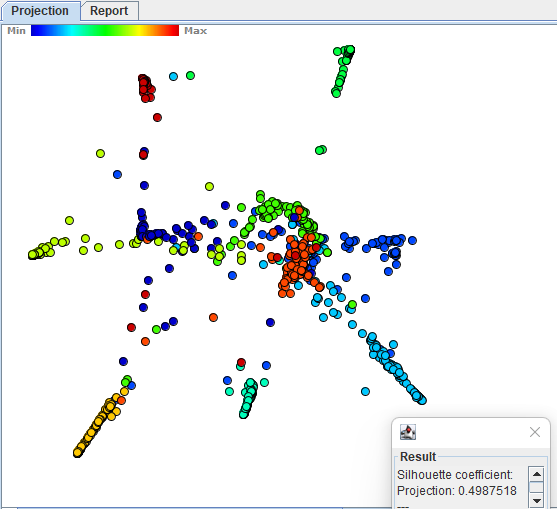
\includegraphics[width=\textwidth]{lsp10.png}}
\vfill
\subfloat
  []
  {\label{fig:lsp100Panel}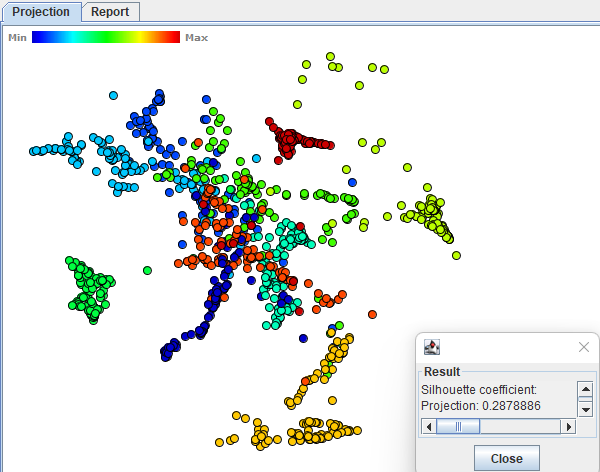
\includegraphics[width=\textwidth]{lsp100.png}}
  \end{minipage}}
\usebox{\measurebox}\qquad
\begin{minipage}[b][\ht\measurebox][s]{.55\textwidth}
\centering
\subfloat
  []
  {\label{fig:lsp5Panel}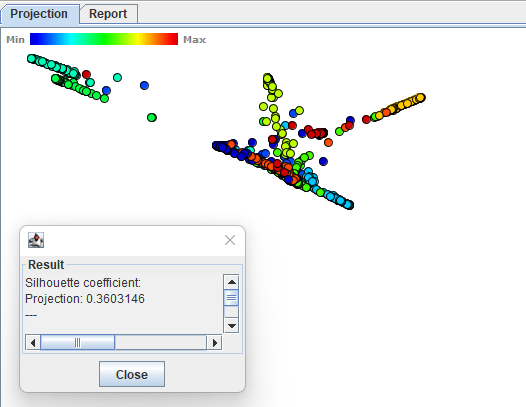
\includegraphics[height=6cm]{lsp5.png}}
\vfill
\subfloat
  []
  {\label{fig:lsp10DtwPanel}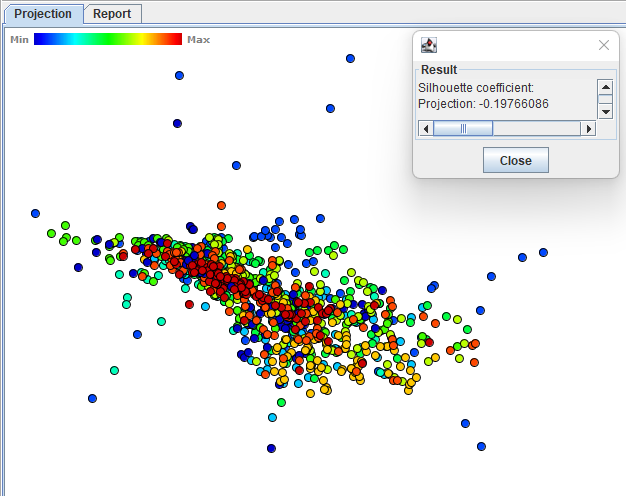
\includegraphics[height=5cm]{lsp10dtw.png}}
\end{minipage}
\caption{(a) LSP with K=10 (b) LSP with K=100 (c) LSP with K=5 (d) LSP with K=10, but DTW distance instead of euclidean distance.}
\label{fig:lsp}
\end{figure}

The results for LSP are interesting, and varied. Firstly, the default value of k (100), led to the points being poorly seperated, and large overlap between groups. When fixing k as the number of classes in the data (10), results improved drastically. Looking at the k=10 version, some categories, e.g. dinosaurs in the top right, mountains in the bottom left, are almost completely isolated from the rest of the groups. We similar issues to NJ, for similar reasons - the similar proportions of the main colours in the images. Some buildings and, beaches are mixed together. Buses and buildings that have similar paint patterns also cause some overlap in the groupings.

An interesting aspect which I experimented with, was the distance measure used. The fact that similarity in colours is heavily rewarded is a consequence of using euclidean distance as a measure of similarity of images - it compares respective pixels in images, which loses any sort of meaningful notion of shape, and naturally heavily rewards large patches of similar colours in images irrespective of the shapes. For this reason, I thought DTW would be interesting to compare against (with k=10), as it accounts for some small local distortions between images, which should at least allow it to incporporate a little more shape-based information. Alas, the results seem to be much poorer, and this is not effective.


\subsubsection*{tsne}

\begin{center}
\begin{figure}
    \centering
	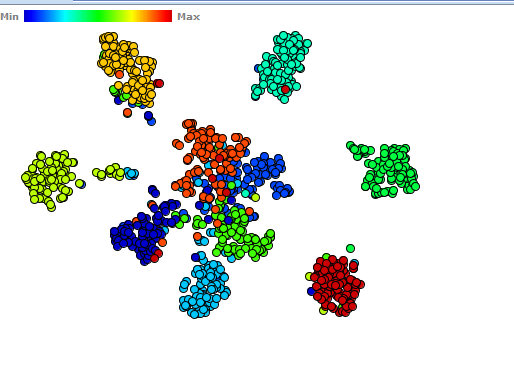
\includegraphics[width=0.95\columnwidth]{tsne.PNG} 
	\caption{T-SNE projection seems even more effective here}
	\label{fig:tsne}
	\end{figure}
\end{center}

\begin{center}
\begin{figure}[H]
    \centering
	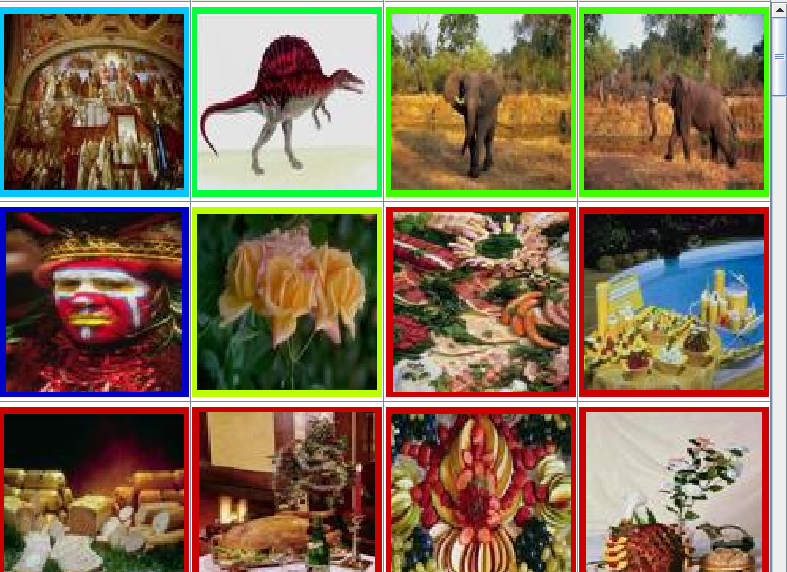
\includegraphics[width=0.95\columnwidth]{tsneConfusion.PNG} 
	\caption{A smaple of images categorised as neighbours in the T-SNE projection, but are from different classes. Notice the similar colours of the images. Silhouette coefficient is 0.4551515.}
	\label{fig:tsneMistakes}
	\end{figure}
\end{center}

The separation here is really good, with a silhouette coefficient of 0.4551515. The groupings are extremely distinct and distant, except for the centre, which has some degree of overlap. Inspecting a portion of this (below), we once again see that this is caused by very similar proportions of colours in neighbouring images.

\subsubsection*{Other methods}

\begin{center}
\begin{figure}[H]
    \centering
	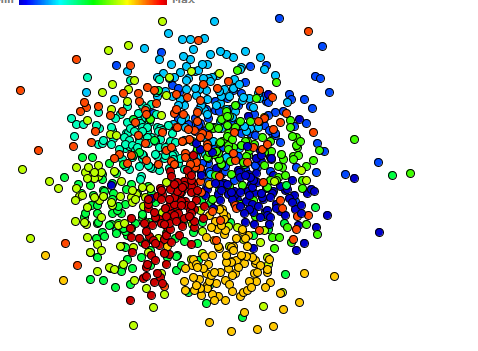
\includegraphics[width=0.95\columnwidth]{sammon.PNG} 
	\caption{Sammon mapping.}
	\label{fig:sammon}
	\end{figure}
\end{center}

\begin{center}
\begin{figure}[H]
    \centering
	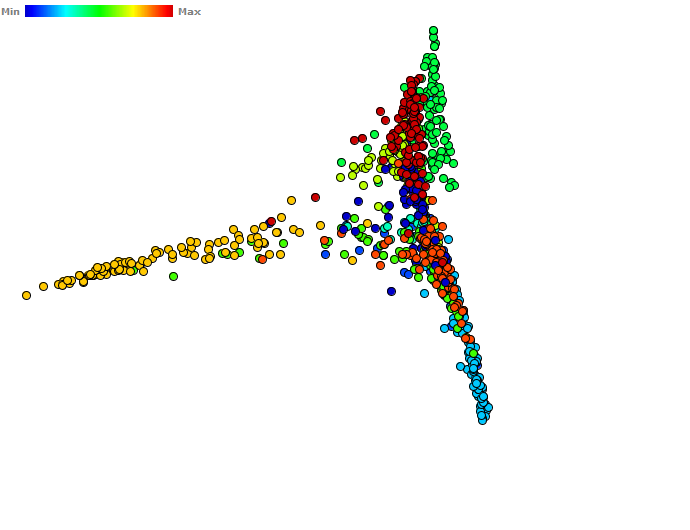
\includegraphics[width=0.95\columnwidth]{pca.PNG} 
	\caption{PCA.}
	\label{fig:pca}
	\end{figure}
\end{center}


\begin{center}
\begin{figure}[H]
    \centering
	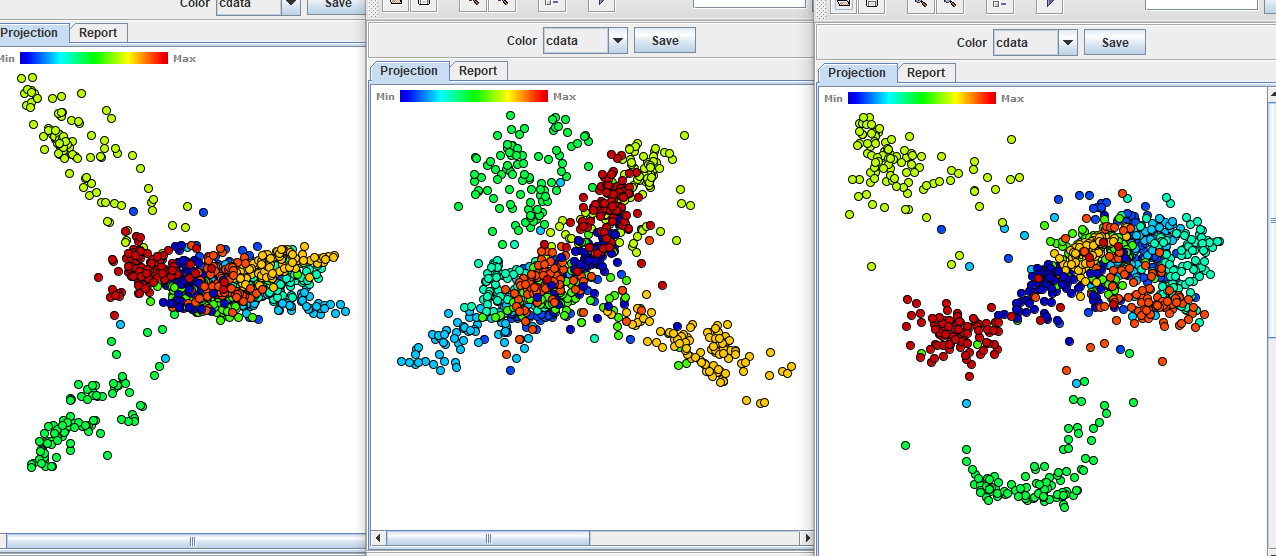
\includegraphics[width=0.95\columnwidth]{isomap.PNG} 
	\caption{ISOMAP.}
	\label{fig:isomap}
	\end{figure}
\end{center}

\begin{center}
\begin{figure}[H]
    \centering
	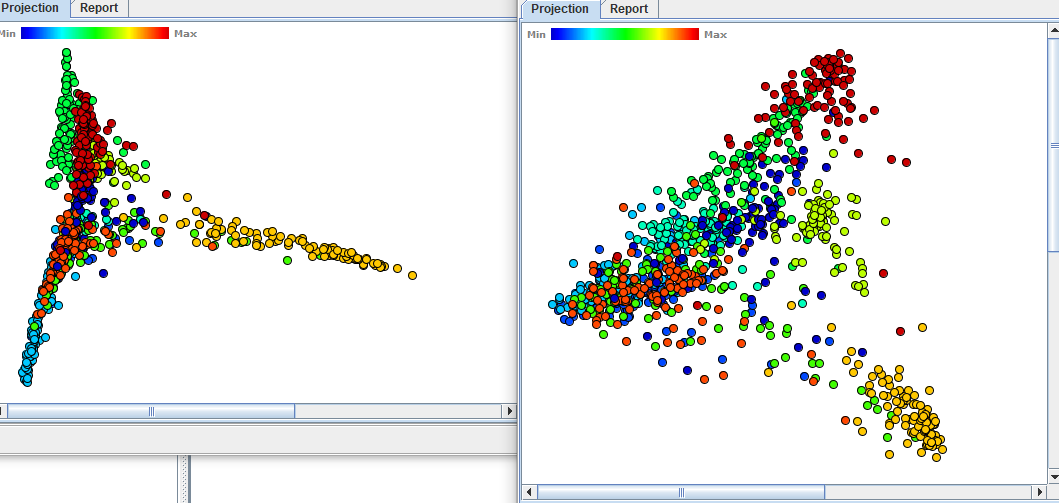
\includegraphics[width=0.95\columnwidth]{mdsEucVSCos.PNG} 
	\caption{MDS, comparing euclidean based distance to cosine based dissimilarity.}
	\label{fig:mdsEuc}
	\end{figure}
\end{center}


Overall, LSP, the Neighbour Joining Radial Tree, and T-SNE seems to give the best results, based on visual inspection. Using silhouette coefficient as a measure of clustering, LSP is deemed the best model to apply here. This stems from the fact that LSP is geared towards cases where the numbers of classes are known - in this case we know that there are 10 fixed classes of interest. Other methods produce results that have high degrees of overlap between classes. Changing the dissimilarity measure to DTW and consine-based measures failed to produce improvements in results.

\subsubsection*{Part B - exploring a document collection}

Based on the performance from the last part, I chose to focus my attention on tuning LSP, T-SNE and the NJ tree.

Below are all the resulting projections, all followed  by interpretation.

\begin{center}
\begin{figure}[H]
    \centering
	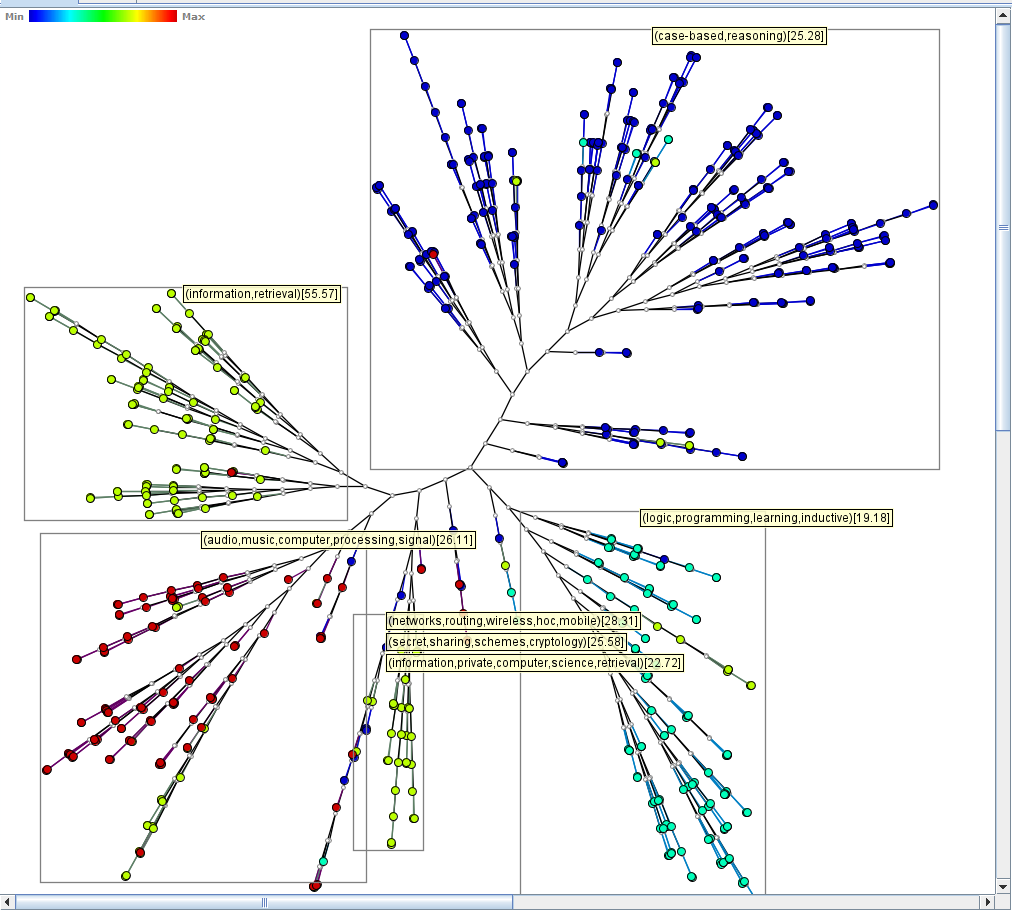
\includegraphics[width=0.55\columnwidth]{neighbourJoiningText.png} 
	\caption{NJ TREE.}
	\label{fig:njtext}
	\end{figure}
\end{center}

\begin{center}
\begin{figure}[H]
    \centering
	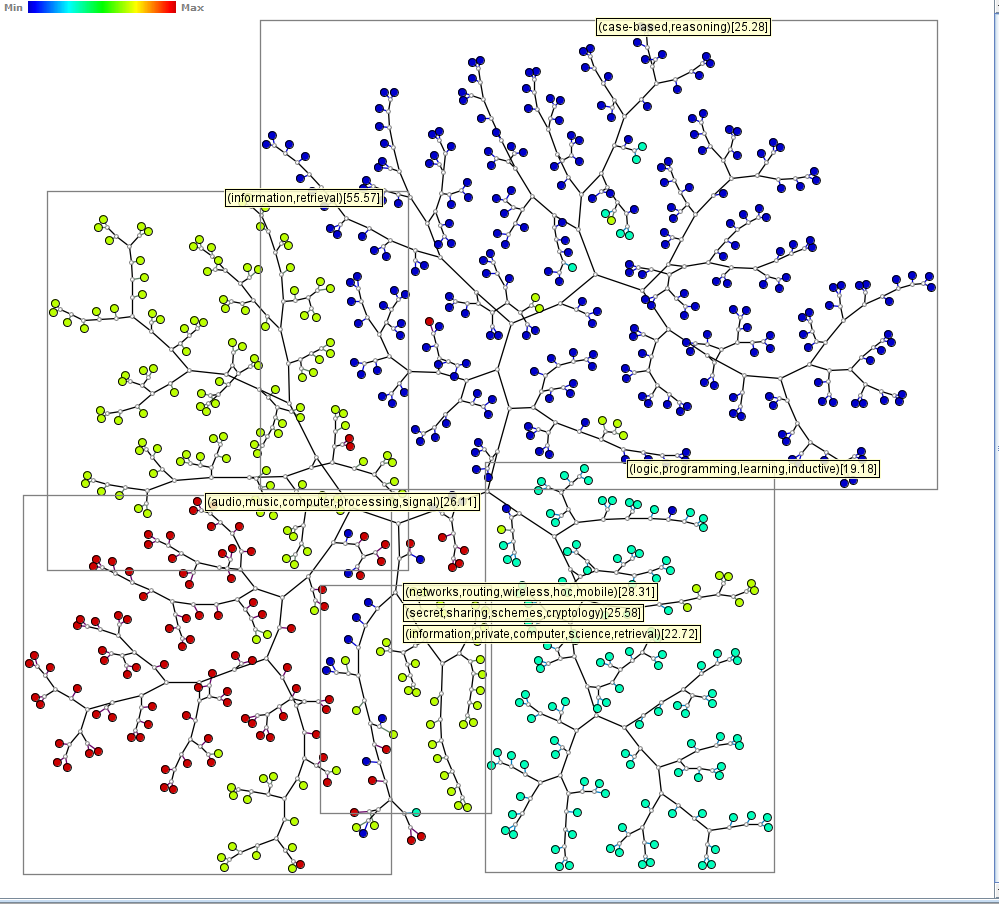
\includegraphics[width=0.55\columnwidth]{forceBasedText.png} 
	\caption{Force based NJ TREE.}
	\label{fig:fbnjtext}
	\end{figure}
\end{center}

\begin{center}
\begin{figure}[H]
    \centering
	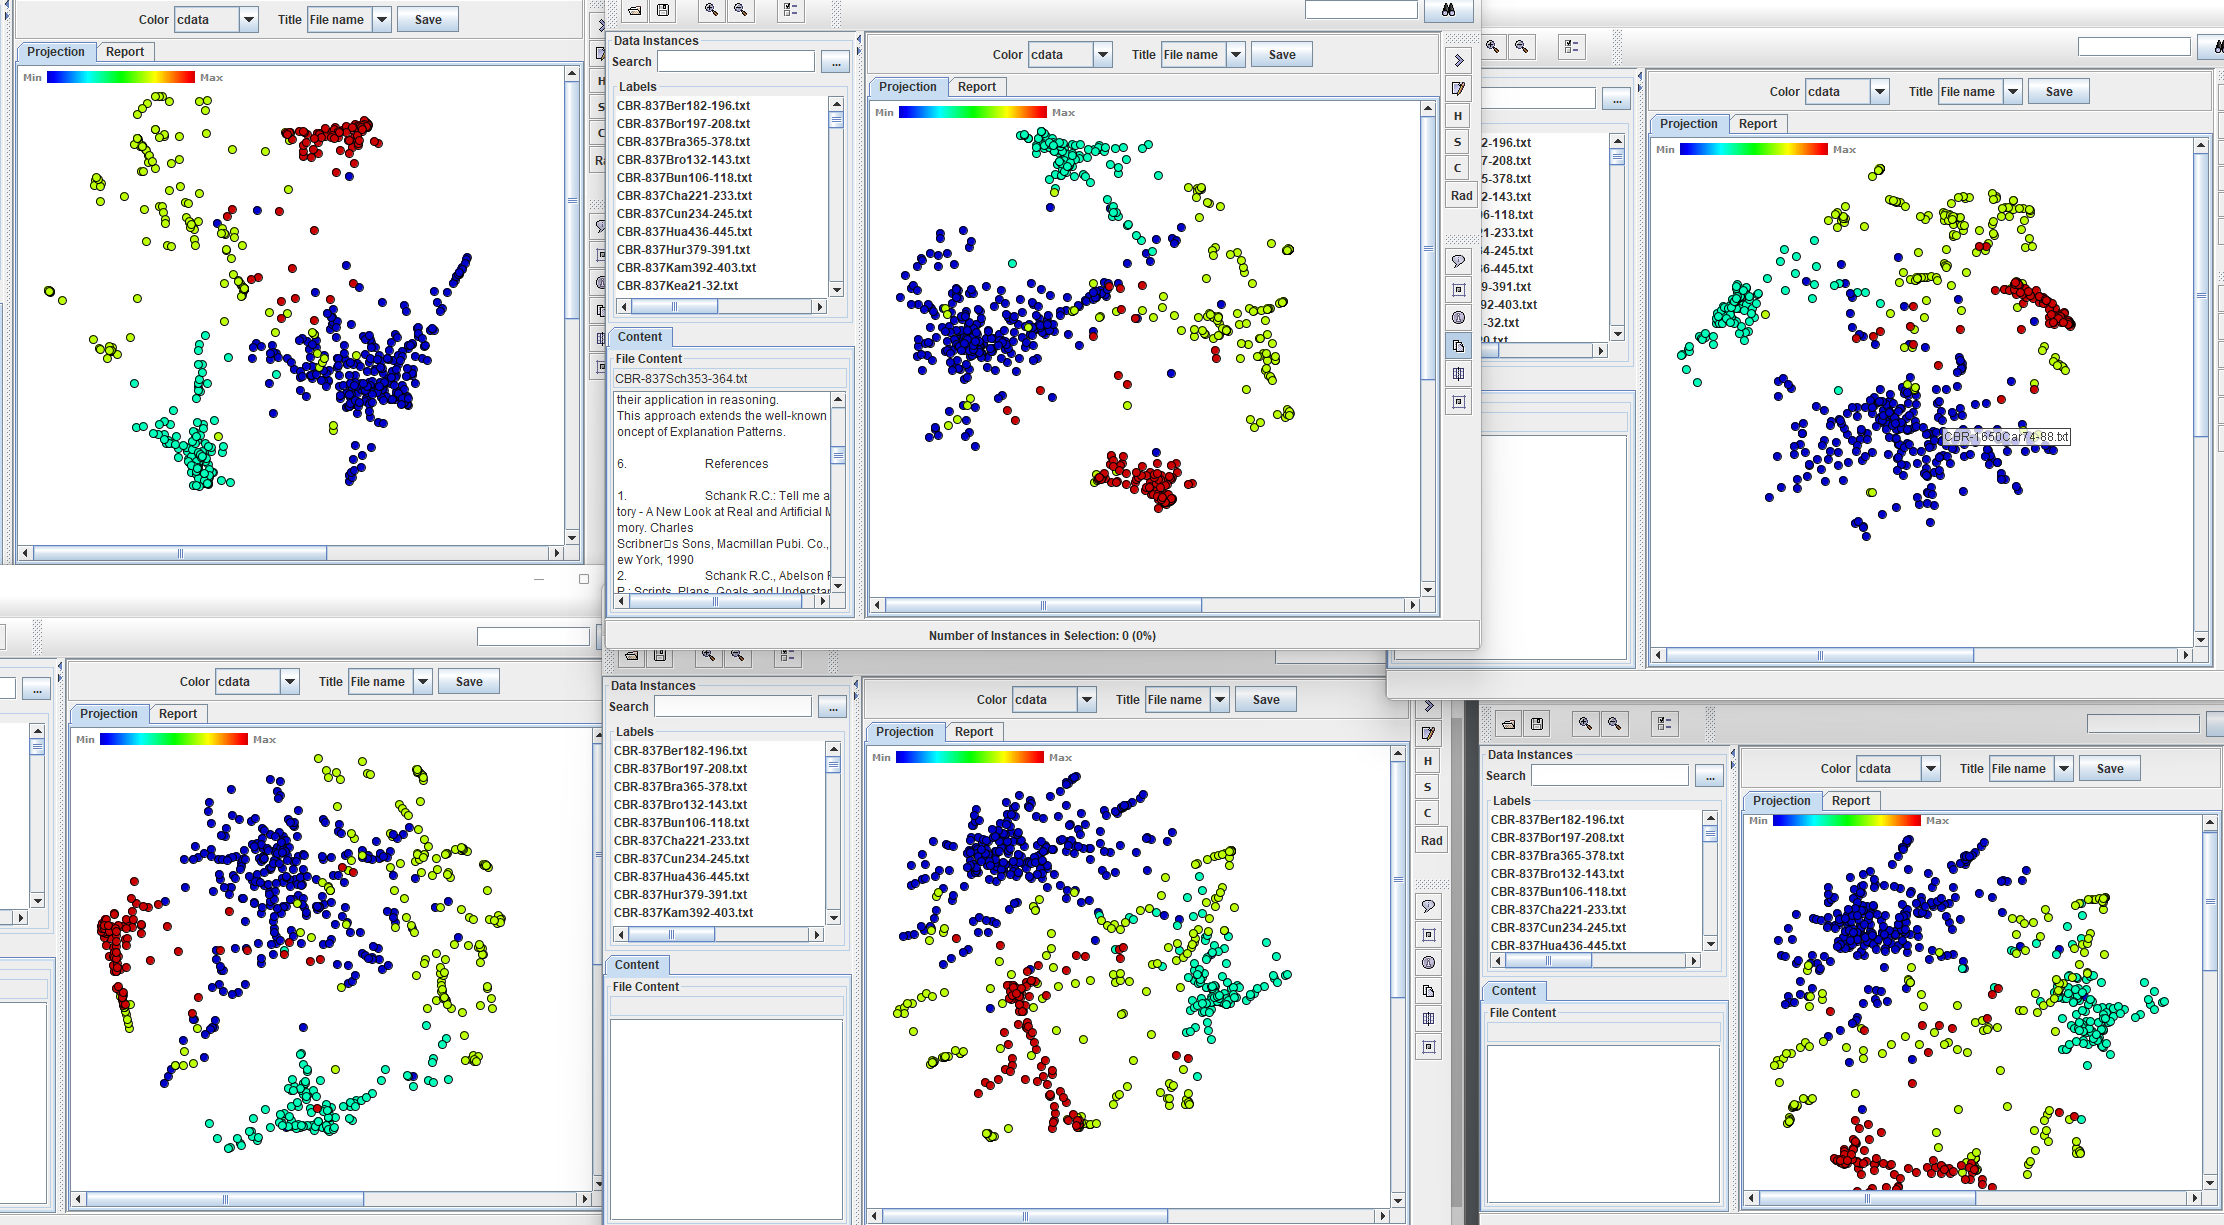
\includegraphics[width=0.85\columnwidth]{lspVaryingKTest.png} 
	\caption{Running LSP with different values for K, ranging from as low as 5 to as high as 70.}
	\label{fig:lspvarying}
	\end{figure}
\end{center}

\begin{center}
\begin{figure}[H]
    \centering
	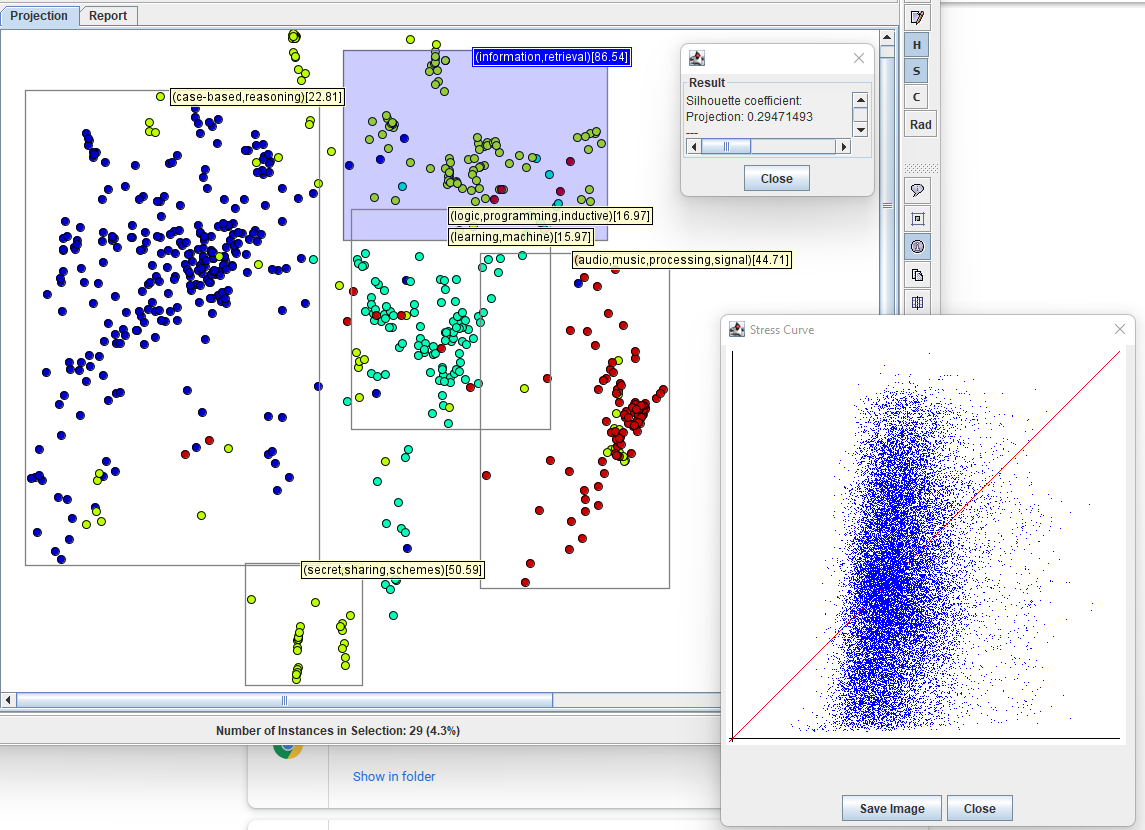
\includegraphics[width=0.55\columnwidth]{LSPtext.png} 
	\caption{Assessing LSP with k=67.}
	\label{fig:lspk67}
	\end{figure}
\end{center}

\begin{center}
\begin{figure}[H]
    \centering
	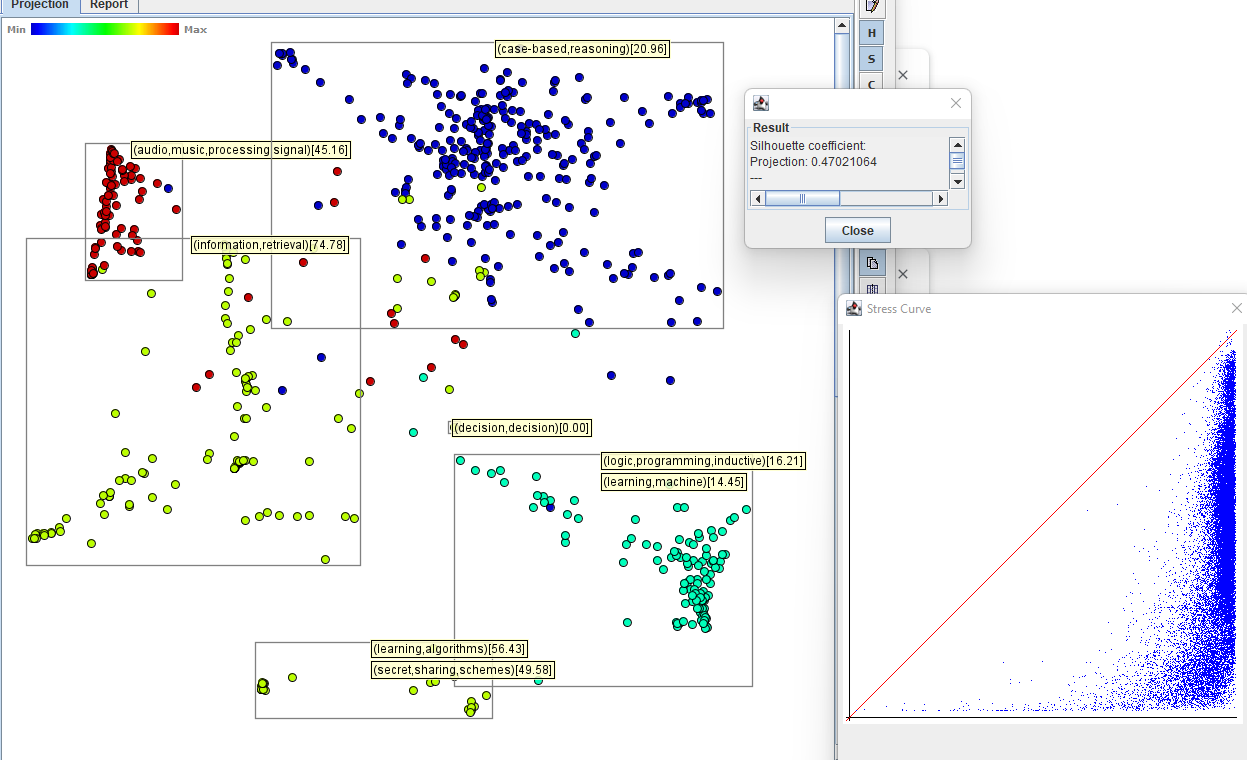
\includegraphics[width=0.55\columnwidth]{LSPtext15classes.png} 
	\caption{Assessing LSP with k=15.}
	\label{fig:lspk15}
	\end{figure}
\end{center}

\begin{center}
\begin{figure}[H]
    \centering
	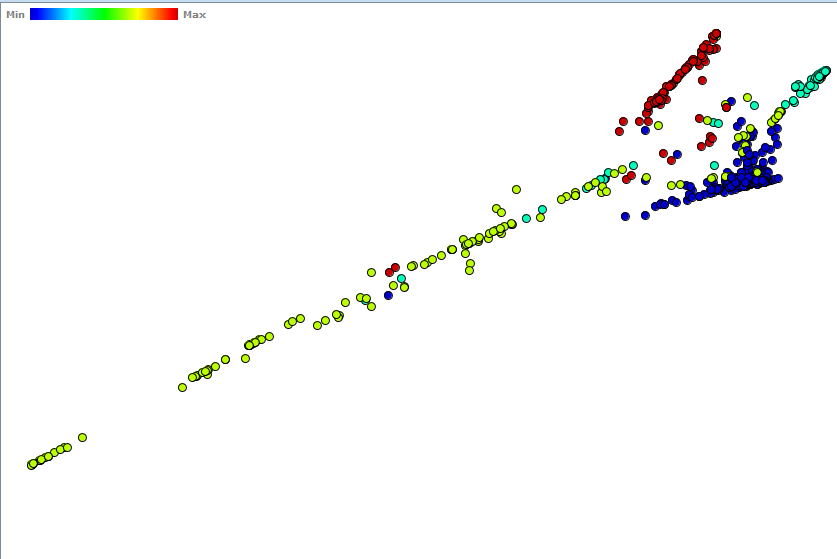
\includegraphics[width=0.55\columnwidth]{lspText5classes.png} 
	\caption{Assessing LSP with k=5.}
	\label{fig:lsp5classes}
	\end{figure}
\end{center}

\begin{center}
\begin{figure}[H]
    \centering
	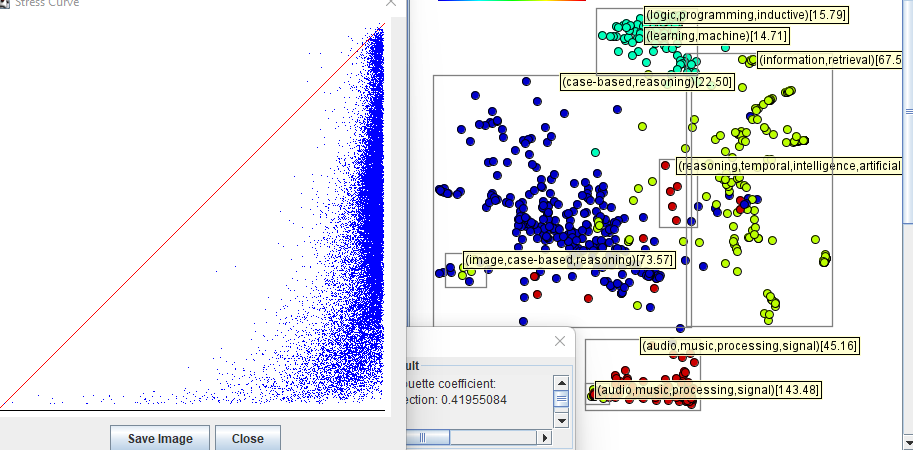
\includegraphics[width=0.55\columnwidth]{lsp34TextBest.png} 
	\caption{Assessing LSP with k=34.}
	\label{fig:bestlsptext}
	\end{figure}
\end{center}



\begin{center}
\begin{figure}[H]
    \centering
	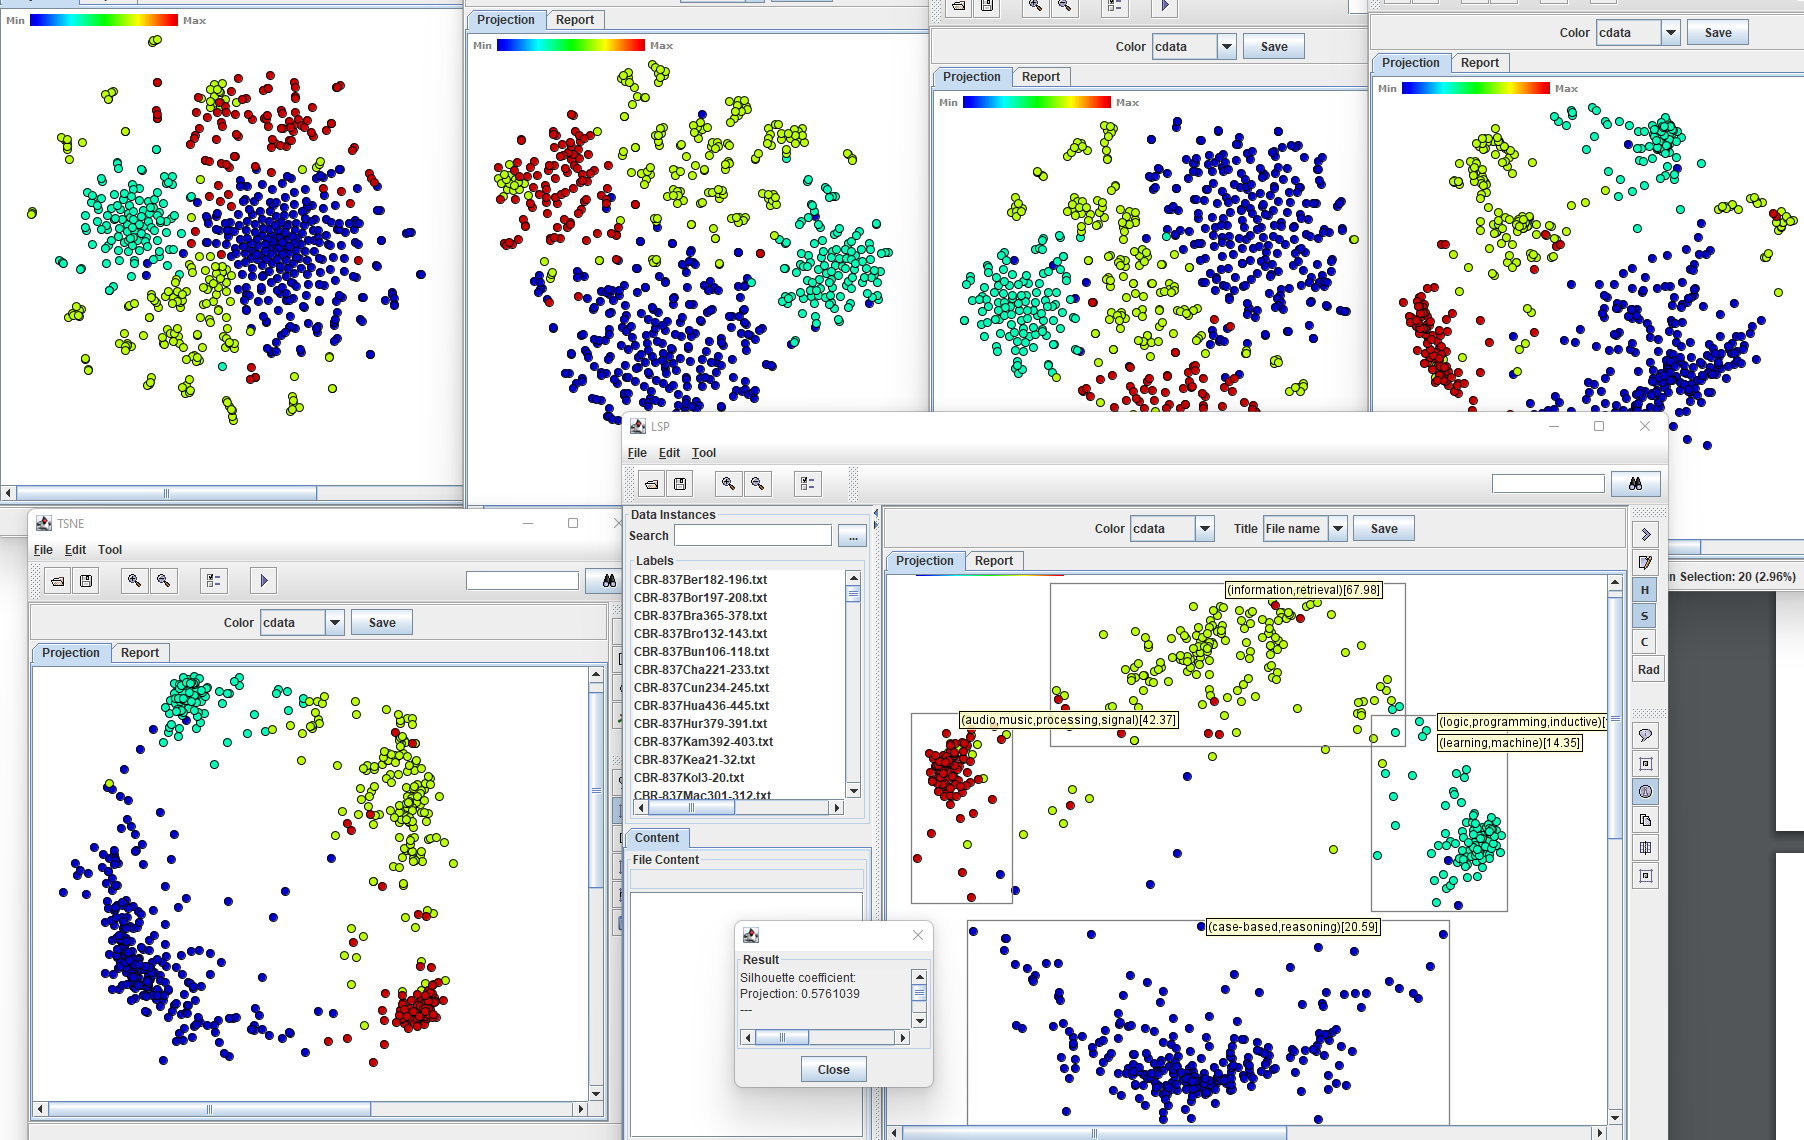
\includegraphics[width=0.85\columnwidth]{tSneupto600.png} 
	\caption{T-SNE with perplexity varying from 30 up to 600.}
	\label{fig:tsneVarying}
	\end{figure}
\end{center}

\begin{center}
\begin{figure}[H]
    \centering
	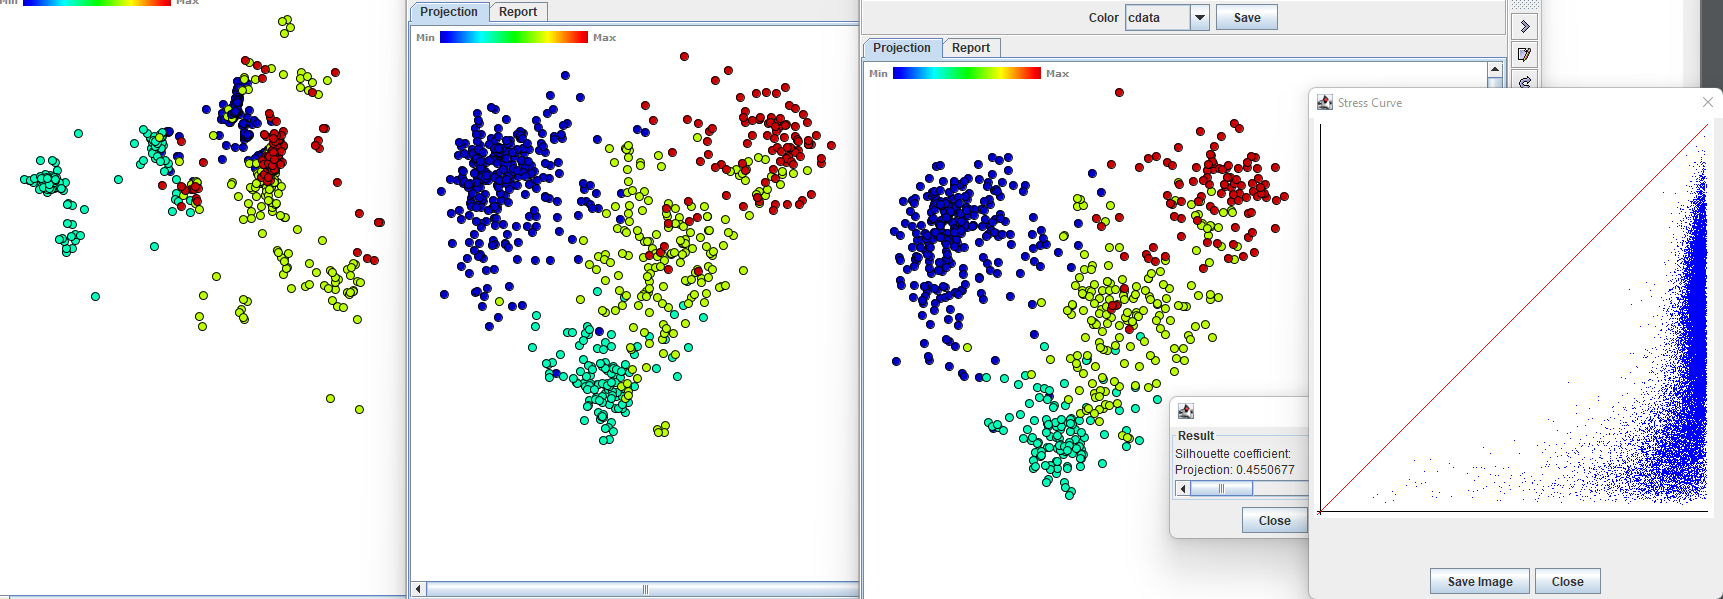
\includegraphics[width=0.85\columnwidth]{isoMap10-15-20.png} 
	\caption{Isomap with the number of neighbours neighbouring from 10 to 15 to 20.}
	\label{fig:isomaptext}
	\end{figure}
\end{center}


The Neighbour Joining tree is highly effective here. On visual inspection, the branches are well separated, with very few incorrectly placed points. Performing force-based placement on this tree leads to a very effective way of identifying and assessing these misplaced points, more about this to follow.

The results of running LSP are good, but not as impressive as the previous section. Interestingly, setting k=5 (the number of labels/classes in the dataset) does not lead to the optimal results as before. Figure \ref{fig:lspvarying} shows LSP running starting with k=5 and working up in rough increments of 15. The best results were a achieved with an intermediate value of roughly k=15. This leads to an initial hypothesis that the differences between the classes in the underlying data is not as distinct as the original data, and that there are wide internal variations inside these classes.

Results of T-SNE are also quite interesting - a high perplexity factor is required to achieve good separation. Interestingly, the silhouette coefficient of the best T-SNE projection (0.57) is significantly better than that of the best LSP projection (0.47).

Isomap performs better with an increased neighbour parameter, and has results slightly worse than LSP, and much worse than T-SNE.

\begin{center}
\begin{figure}[H]
    \centering
	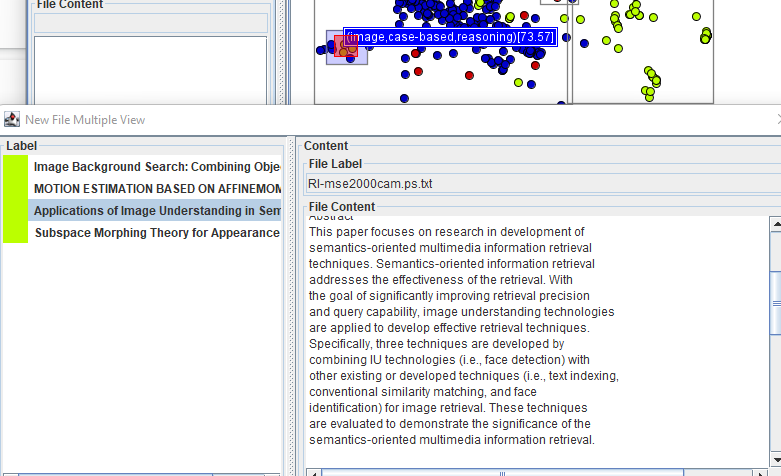
\includegraphics[width=0.85\columnwidth]{example overlap text lsp.png} 
	\caption{An example of a small group of \textit{information retrieval} category atricles that were mis-categroised with case-based reasoning articles by LSP.}
	\label{fig:mixeduptext}
	\end{figure}
\end{center}

The actual articles that were miscategorised, or bordered multiple clusters were very similar between all methods. An example of a small group of very poorly placed articles for an application of LSP (k=34) is shown above, that illustrates this point well. The example shows articles that are categorised as belonging to the domain of information retrieval, but clearly involve aspects and components of case based reasoning articles. This is indicative of a crucial difference between this text analysis and the previous image analysis - in general, an image of food is an image of food, and nothing else. The delineation is not necessarily as clear when it comes to research papers - papers in one domain may contain aspects of, techniques from or applications to other domains. This makes the underlying labelling of the data much less reliable and concrete, hugely limiting the potential for well-segmented projections. From this observation, it makes sense that T-SNE performs better than LSP as it does not rely on a hard-coded number of clusters, since even and ideal clustering of the data has blurred edges (where there is overlap in domains). For practical purposes, I believe that the force-based placed neighbour joining tree (figure \ref{fig:fbnjtext}) is likely the best to use to explore the dataset. This is because the spacing of the branches allows us to much more easily identify the ``confused'' groupings within other categories, e.g. information retrieval articles in the machine learning domain, and assess what is causing their miscategorisation, which is of great importance to understand before employing the use of this dataset in any real-world application.


\subsubsection*{Part C - exploring other datasets}

\vspace{0.5cm} 

\textbf{Reuters news data}

\begin{center}
\begin{figure}[H]
    \centering
	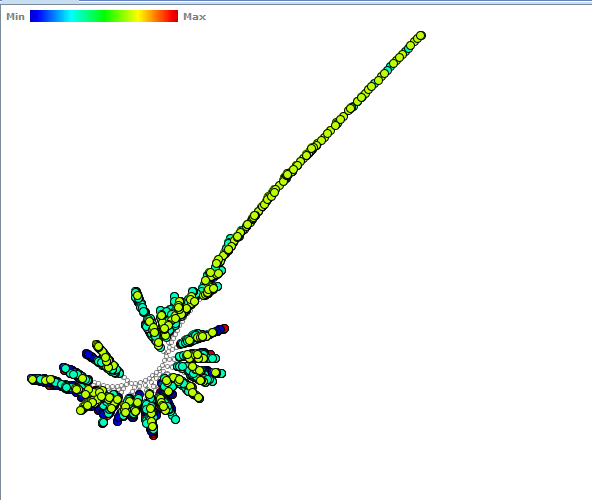
\includegraphics[width=0.65\columnwidth]{task2c/reutersNJ.PNG} 
	\caption{Neighbourhood Joining tree on the Reuters news data}
	\label{fig:retunj}
	\end{figure}
\end{center}

\begin{center}
\begin{figure}[H]
    \centering
	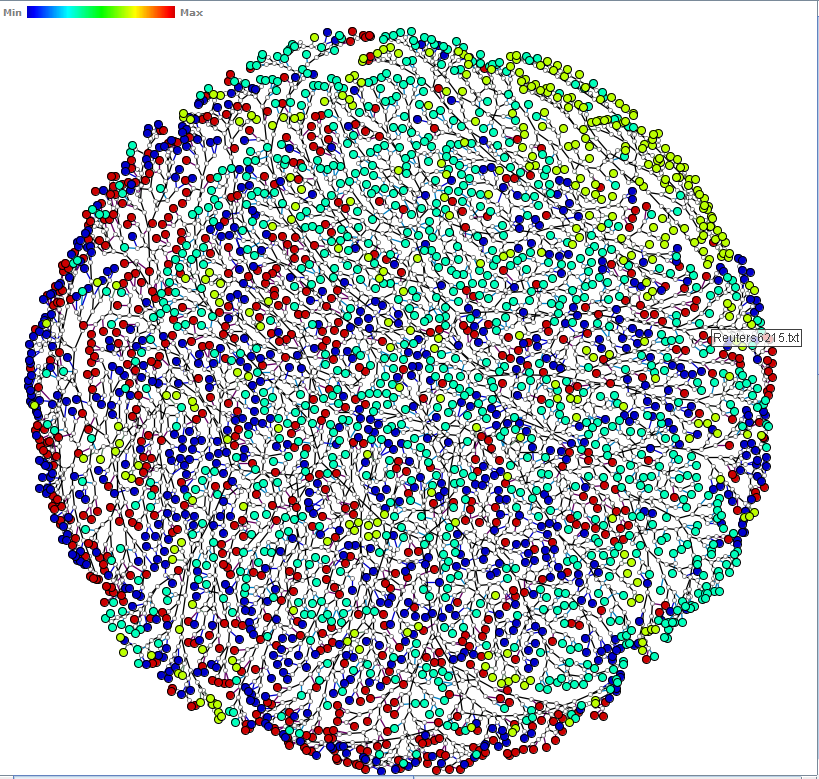
\includegraphics[width=0.65\columnwidth]{task2c/reutersNJ-FB.PNG} 
	\caption{Force based distance applied to neighbourhood Joining tree on the Reuters news data}
	\label{fig:retunjfb}
	\end{figure}
\end{center}


\begin{center}
\begin{figure}[H]
    \centering
	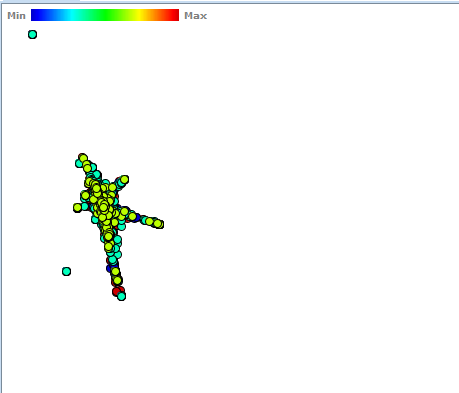
\includegraphics[width=0.65\columnwidth]{task2c/reutersLSP-k5-N7.PNG}
	\caption{LSP k=5, neighbours=7}
	\label{fig:reutlsp5.7}
	\end{figure}
\end{center}

\begin{center}
\begin{figure}[H]
    \centering
	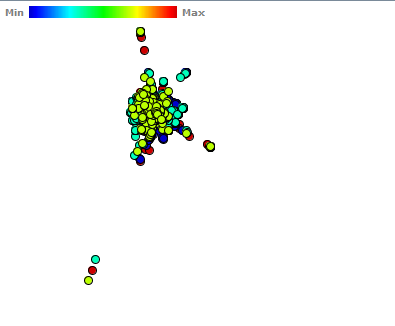
\includegraphics[width=0.65\columnwidth]{task2c/reutersLSP-k30.PNG}
	\caption{LSP k=30}
	\label{fig:reutlsp30}
	\end{figure}
\end{center}

\begin{center}
\begin{figure}[H]
    \centering
	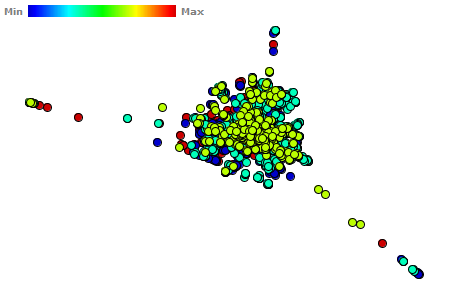
\includegraphics[width=0.65\columnwidth]{task2c/reutersLSP-k60.PNG}
	\caption{LSP k=60}
	\label{fig:reutlsp60}
	\end{figure}
\end{center}

\begin{center}
\begin{figure}[H]
    \centering
	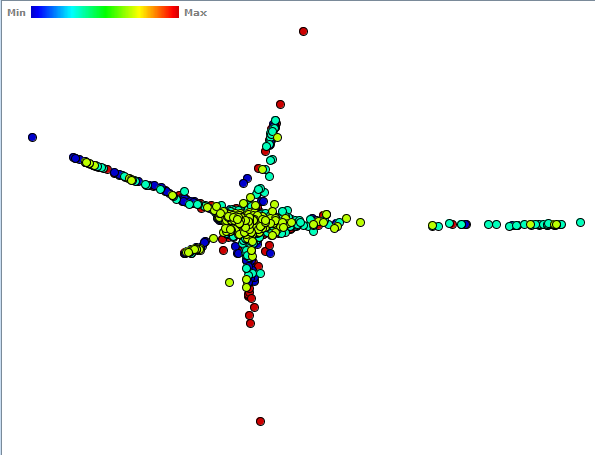
\includegraphics[width=0.65\columnwidth]{task2c/reutersLSP-k65-N60.PNG}
	\caption{LSP k=5, neighbours=60}
	\label{fig:reutlsp66.60}
	\end{figure}
\end{center}

\begin{center}
\begin{figure}[H]
    \centering
	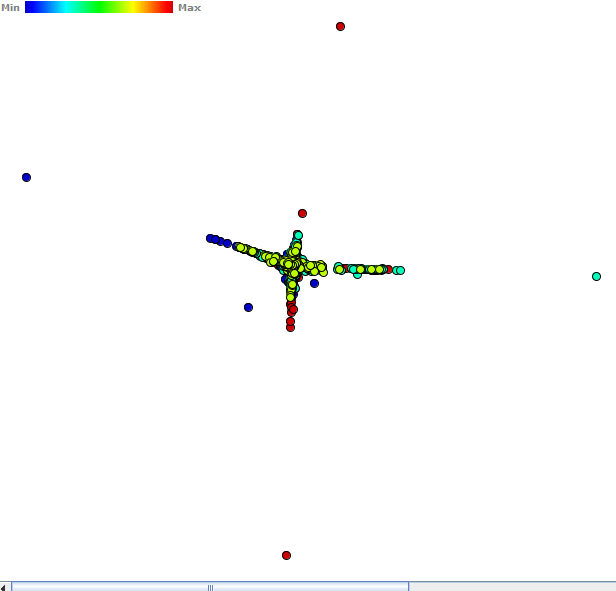
\includegraphics[width=0.65\columnwidth]{task2c/reutersLSP-k65-N100.PNG}
	\caption{LSP k=5, neighbours=100}
	\label{fig:reutlsp65.100}
	\end{figure}
\end{center}

\begin{center}
\begin{figure}[H]
    \centering
	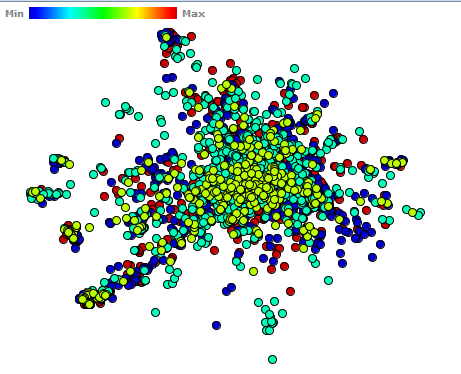
\includegraphics[width=0.65\columnwidth]{task2c/reutersLSP-k100-N20.PNG}
	\caption{LSP k=100, neighbours=20}
	\label{}
	\end{figure}
\end{center}

\begin{center}
\begin{figure}[H]
    \centering
	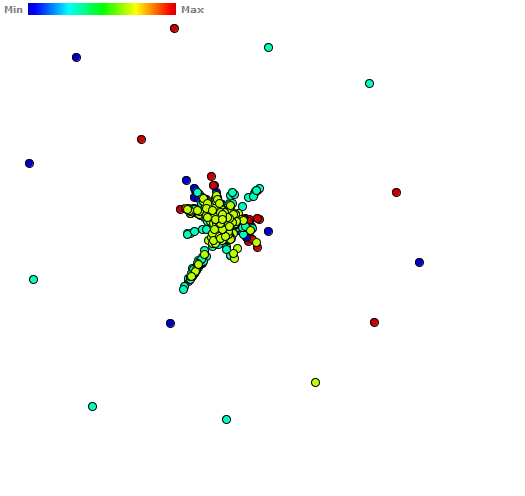
\includegraphics[width=0.65\columnwidth]{task2c/reutersK15N100.PNG}
	\caption{LSP k=15, neighbours=100}
	\label{fig:reutlsp15.100}
	\end{figure}
\end{center}


\begin{center}
\begin{figure}[H]
    \centering
	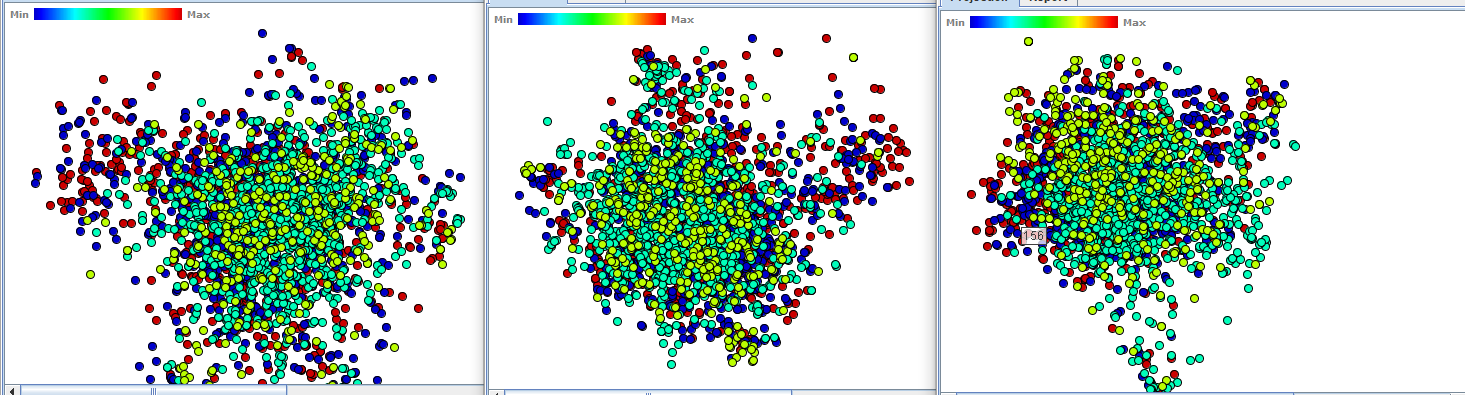
\includegraphics[width=0.65\columnwidth]{task2c/reutersISOMAP.PNG}
	\caption{ISOMAP under a range of neighbour parameters}
	\label{fig:reutisomap}
	\end{figure}
\end{center}

\begin{center}
\begin{figure}[H]
    \centering
	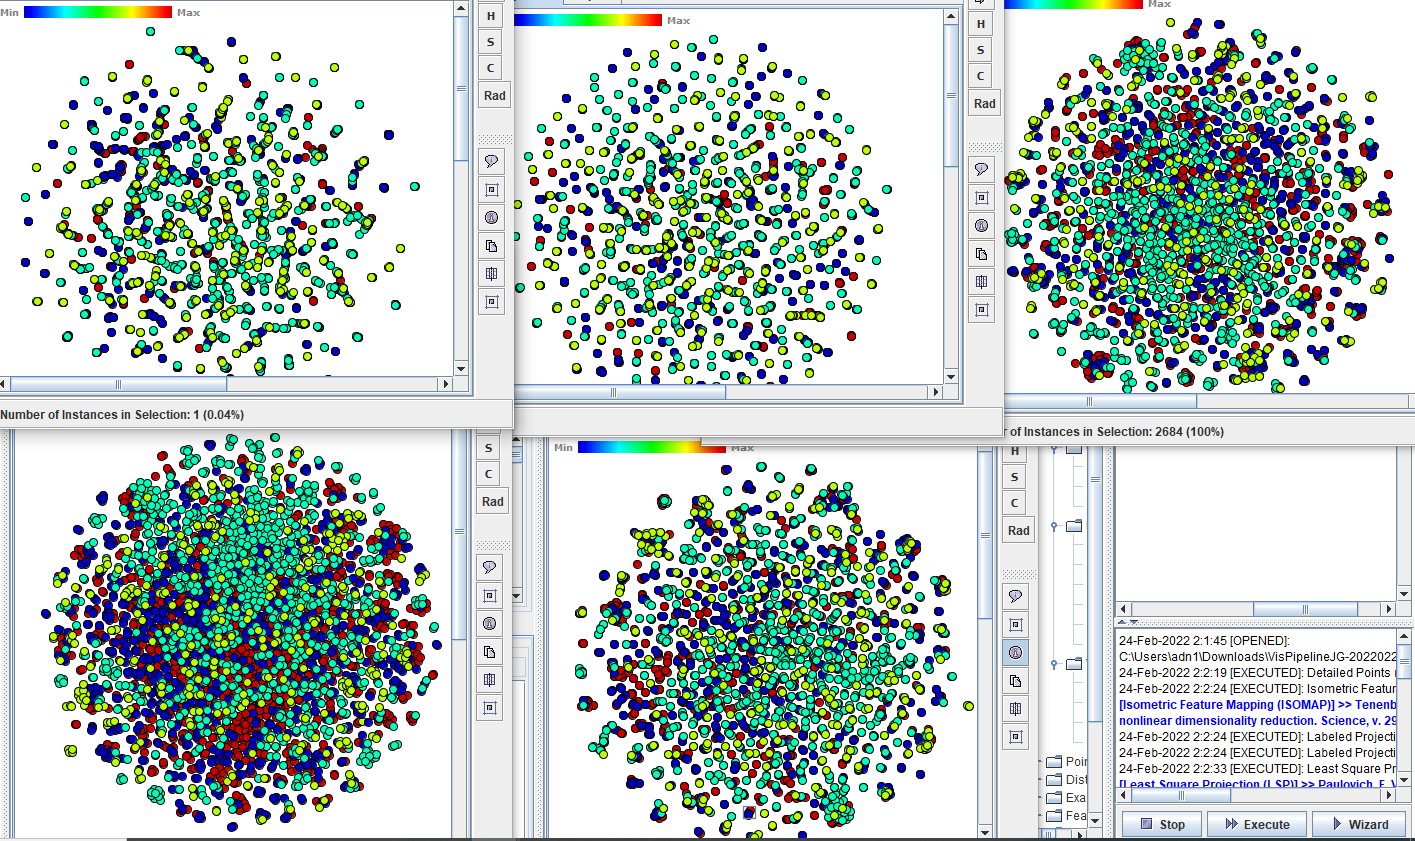
\includegraphics[width=0.65\columnwidth]{task2c/reutersTSNE.PNG}
	\caption{TSNE, with perplexity ranging from 5 to 600}
	\label{fig:reuttsneCOS}
	\end{figure}
\end{center}

\begin{center}
\begin{figure}[H]
    \centering
	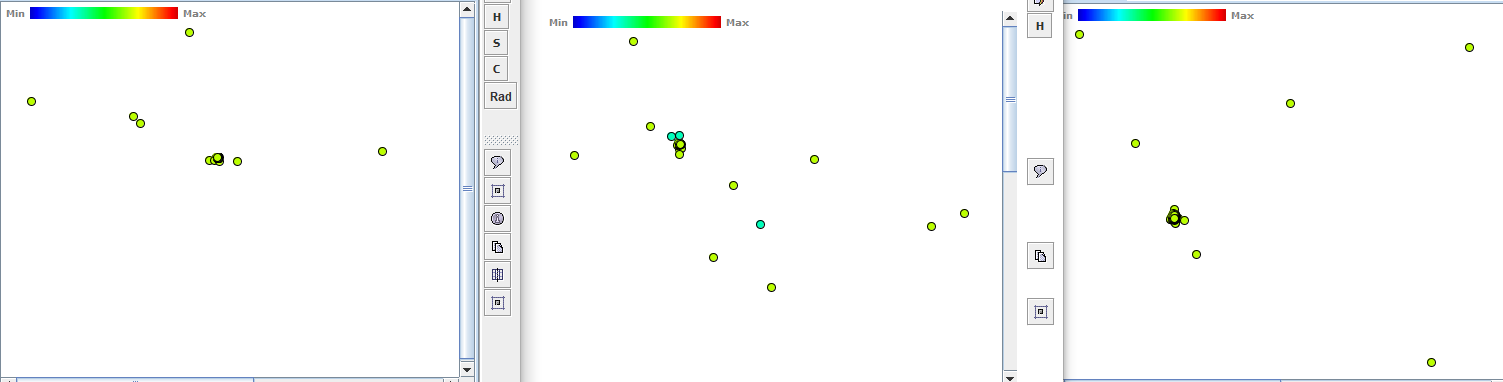
\includegraphics[width=0.65\columnwidth]{task2c/reutersTSNE-EUC-5,100,500.PNG}
	\caption{TSNE with Euclidean distance, where the previous projections were performed with cosine based dissimilarity measures.}
	\label{fig:reuttsneeuc}
	\end{figure}
\end{center}

Projecting this data is much more challenging. This seems to suffer from a similar problem to the CBR dataset, but to a much higher extent, leading to a conclusion that there is a great deal of overlap between articles on supposedly distinct topics. Interestingly, LSP seems to perform much better - under an optimal choice of k - than T-SNE. This seems to be by forcing the points apart into 5 distinct groups, which may not be very easy to notice arising naturally out of the data. After assessing many values of k, values around 5 seemed to give the best results, with very high values for the amount of neighbours to consider, which seems to help force the points apart. There is still a large degree of overlap, but distinct ``arms'' can be see emerging from a mixed centre in the data. All other methods seemed to result in well-mixed, unclustered masses, regardless of the parameters chosen. I will now assess the LSP, K=5 projection to assess which articles are clustered together, which are mixed, and why.

\begin{center}
\begin{figure}[H]
    \centering
	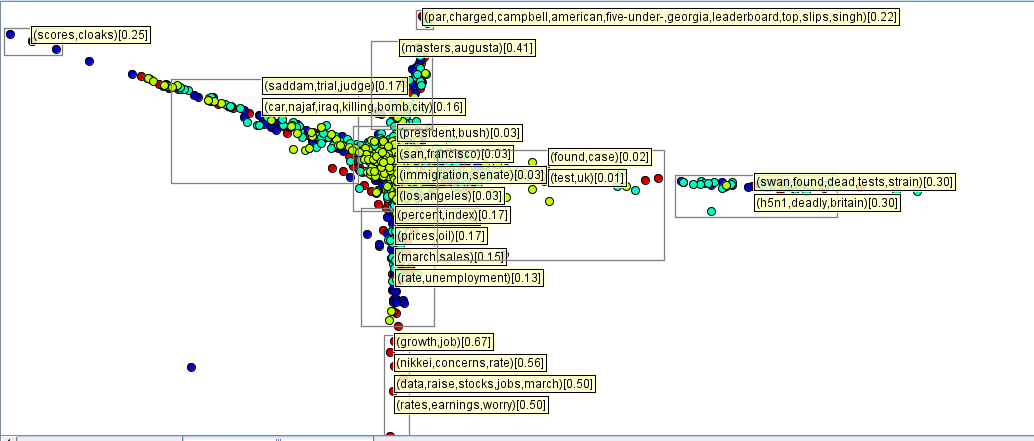
\includegraphics[width=0.65\columnwidth]{task2c/explainingReuters.PNG}
	\caption{What are the main topics in the confused articles?}
	\label{fig:explReuters}
	\end{figure}
\end{center}

Exploring the projection, it becomes clear that the centre of the mass of points seems to correspond to American news, about America. Almost all of the articles \textit{involve} America, and it seems that the less the article is \textbf{about} America in general, the more easily segmented it is - e.g. invasion of Iraq and bird flu are easier to segment than articles about current affairs in San Francisco.


\vspace{1cm}

\textbf{EXPLORING ANOTHER IMAGE DATASET}

\vspace{1cm}

For variety, I decided in this section to consider another image dataset - specifically ``Medical  12 class''.

\begin{center}
\begin{figure}[H]
    \centering
	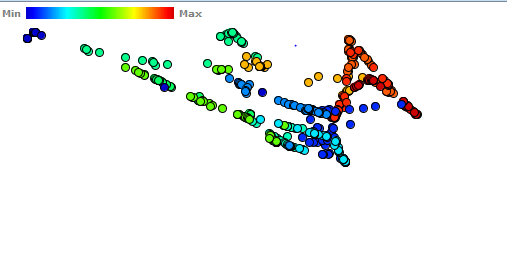
\includegraphics[width=0.65\columnwidth]{task2d/medLSP12-10.PNG}
	\caption{LSP k=12, N=10}
	\label{fig:med1210}
	\end{figure}
\end{center}

\begin{center}
\begin{figure}[H]
    \centering
	\includegraphics[width=0.65\columnwidth]{task2d/medLSP12-50.PNG}
	\caption{LSP k=12, N=50}
	\label{fig:med1250}
	\end{figure}
\end{center}

\begin{center}
\begin{figure}[H]
    \centering
	\includegraphics[width=0.65\columnwidth]{task2d/medLSP12-75.PNG}
	\caption{LSP k=12, N=75}
	\label{fig:med12175}
	\end{figure}
\end{center}

\begin{center}
\begin{figure}[H]
    \centering
	\includegraphics[width=0.65\columnwidth]{task2d/medLSP12-100.PNG}
	\caption{LSP k=12, N=100}
	\label{fig:med12100}
	\end{figure}
\end{center}

\begin{center}
\begin{figure}[H]
    \centering
	\includegraphics[width=0.65\columnwidth]{task2d/medLSP15-100-COS.PNG}
	\caption{LSP k=15, N=100, Cosine Dissimilarity}
	\label{fig:med1275}
	\end{figure}
\end{center}


\begin{center}
\begin{figure}[H]
    \centering
	\includegraphics[width=0.65\columnwidth]{task2d/medTSNE5.PNG}
	\caption{TSNE, perplexity 5}
	\label{fig:medt5}
	\end{figure}
\end{center}


\begin{center}
\begin{figure}[H]
    \centering
	\includegraphics[width=0.65\columnwidth]{task2d/medTSNE10.PNG}
	\caption{TSNE, perplexity 10 - silhouette coefficient 0.12}
	\label{fig:medt10}
	\end{figure}
\end{center}

\begin{center}
\begin{figure}[H]
    \centering
	\includegraphics[width=0.65\columnwidth]{task2d/medTSNE10-EUC.PNG}
	\caption{TSNE, perplexity 10, Euclidean distance rather than Cosine-based}
	\label{fig:medt10Euc}
	\end{figure}
\end{center}

\begin{center}
\begin{figure}[H]
    \centering
	\includegraphics[width=0.65\columnwidth]{task2d/medTSNE20.PNG}
	\caption{TSNE, perplexity 20 - silhouette coefficient 0.10}
	\label{fig:medt20}
	\end{figure}
\end{center}

\begin{center}
\begin{figure}[H]
    \centering
	\includegraphics[width=0.65\columnwidth]{task2d/medTSNE30.PNG}
	\caption{TSNE, perplexity 30}
	\label{fig:medt30}
	\end{figure}
\end{center}

\begin{center}
\begin{figure}[H]
    \centering
	\includegraphics[width=0.65\columnwidth]{task2d/medTSNE50.PNG}
	\caption{TSNE, perplexity 50}
	\label{fig:med50}
	\end{figure}
\end{center}

LSP seems to be quite ineffective here, under all sets of trialed parameters - datapoints seem to be flattened into a line, with little effective separation between classes.

TSNE is much more effective, although the results are not perfect at first glance. For all choices of parameters, there is noticeable mixing of classes. Higher perplexity factors tend to result in poor separation, and lower perplexity values tend to result in many over-dispersed clusters, with no middle ground. Based on computed silhouette coefficients, it seems that cosine based dissimilarity is the most effective dissimilarity measure, and 10 the most appropriate perplexity factor.

\begin{center}
\begin{figure}[H]
    \centering
	\includegraphics[width=0.45\columnwidth]{task2d/medNJ.PNG}
	\caption{Neighbour joining tree - quoted silhouette of 0.06, but this seems to be an unreliabel measure for trees}
	\label{fig:medNJ}
	\end{figure}
\end{center}

\begin{center}
\begin{figure}[H]
    \centering
	\includegraphics[width=0.65\columnwidth]{task2d/medNJFB.PNG}
	\caption{Neighbour joining tree with force based placement}
	\label{fig:medNJFB}
	\end{figure}
\end{center}

Creating a neighbour joining tree, we see quite a good separation of classes - although silhouette seems to not be a very effective measure of this. Performing force bases placement also helps present this in a manner that allows anomalous placements of points to be identified, similarly to the previous case. Inspecting these misclassified points helps us draw insights about the aspects of the data that cause difficulties in the previous projection algorithms.

\begin{figure}[H]
\centering
\sbox{\measurebox}{%
  \begin{minipage}[b]{.45\textwidth}
  \subfloat
  []
  {\label{fig:medMisclass1}\includegraphics[width=1\textwidth]{task2d/medMisclass1.PNG}}
\vfill
\subfloat
  []
  {\label{fig:medmissclass2}\includegraphics[width=1\textwidth]{task2d/medMisclass2.PNG}}
  \end{minipage}}
\usebox{\measurebox}\qquad
\begin{minipage}[b][\ht\measurebox][s]{.45\textwidth}
\centering
\subfloat
  []
  {\label{fig:medMisclass3}\includegraphics[width=0.8\textwidth]{task2d/medMisclass3.PNG}}
\vfill
\subfloat
  []
  {\label{fig:medmisclass4}\includegraphics[width=0.8\textwidth]{task2d/medMisclass4.PNG}}
\end{minipage}
\caption{Examples of groups of images that were misclassisfied as being similar}
\label{fig:medmisclass}
\end{figure}

Figure \ref{fig:medmisclass} shows examples of images that were incorrectly grouped by the neighbour joining algorithm. We notice that, for tile (d), the difference between the categories is very nuance, and at first glance, even imperceptible. In tile (a) we see gradual differences between the images - determining whether a scan is of a photo is classes as a scan of the head or spine is somewhat of a grey area depending on how high or low the image is taken relative to the head. Similarly, panel (c) shows this same effect with parts of the brain. Panel (b) shows the last type of miscategroisation, that was in the minority - scans of entirely differentbody parts that were grouped together.


\subsubsection*{Part D - exploring HDI}

I created a .data file, as per the documentation on canvas.  

\begin{center}
\begin{figure}[H]
    \centering
	\includegraphics[width=0.65\columnwidth]{hdiProj/hdiNJ.PNG}
	\caption{Neighbour joining tree}
	\label{fig:hdiNJ}
	\end{figure}
\end{center}

\begin{center}
\begin{figure}[H]
    \centering
	\includegraphics[width=0.45\columnwidth]{hdiProj/hdiNJFB.PNG}
	\caption{Neighbour joining tree with force based placement}
	\label{fig:hdiNJFB}
	\end{figure}
\end{center}

\begin{center}
\begin{figure}[H]
    \centering
	\includegraphics[width=0.65\columnwidth]{hdiProj/hdiLsp3-5.PNG}
	\caption{LSP k=3, neighbours=5}
	\label{fig:hdiLSP3-5}
	\end{figure}
\end{center}

\begin{center}
\begin{figure}[H]
    \centering
	\includegraphics[width=0.65\columnwidth]{hdiProj/hdiLSP-4-5.PNG}
	\caption{LSP k=4, neighbours=5}
	\label{fig:hdiLSP-4-5}
	\end{figure}
\end{center}

\begin{center}
\begin{figure}[H]
    \centering
	\includegraphics[width=0.65\columnwidth]{hdiProj/hdiLSP-4-10.PNG}
	\caption{LSP k=4, neighbours=10}
	\label{fig:hdiLSP-4-10}
	\end{figure}
\end{center}

\begin{center}
\begin{figure}[H]
    \centering
	\includegraphics[width=0.65\columnwidth]{hdiProj/hdiLSP-50-10.PNG}
	\caption{LSP k=50, neighbours=10}
	\label{fig:hdiLSP-50-10}
	\end{figure}
\end{center}

\begin{center}
\begin{figure}[H]
    \centering
	\includegraphics[width=0.65\columnwidth]{hdiProj/hdiTSNE-5.PNG}
	\caption{TSNE perplexity=5}
	\label{fig:hdiTSNE5}
	\end{figure}
\end{center}

\begin{center}
\begin{figure}[H]
    \centering
	\includegraphics[width=0.45\columnwidth]{hdiProj/hdiTSNE-10.PNG}
	\caption{TSNE perplexity=10}
	\label{fig:hdiTSNE10}
	\end{figure}
\end{center}

\begin{center}
\begin{figure}[H]
    \centering
	\includegraphics[width=0.65\columnwidth]{hdiProj/hdiTSNE-15.PNG}
	\caption{TSNE perplexity=15}
	\label{fig:hdiTSNE15}
	\end{figure}
\end{center}

Interestingly, it seems that projections of the HDI data leads to much more linear plots, for the Neighbour Joining Tree, LSP, and T-SNE, under different parameters. These results are quite uninteresting.

Figures  \ref{fig:hdiTSNE5} and \ref{fig:hdiTSNE10} do show interesting behaviour, however - with figure \ref{fig:hdiTSNE5} showing interesting segmented strips. It seems that there are still linear groupings, implying a gradual progression in development between countries. There are distinct groupings, however, implying that the predominant developmental indicators differ between these groups. Figure \ref{fig:hdiTSNE10} is similar, but contains only two groupings.


\section*{Conclusions}

This serves as an extremely brief summary of the key insights above, and is not a substitute for reading the parts themselves.

\subsection{Task 1}

In task 1, I came to a few conclusions both about data visualisation as a technique, and by using it, from the HDR data.

\begin{enumerate}
    \item I found that using a 3D surface plot was far more effective than an animated map over time - by extension, if possible, the use of a time dimension in visualisations should be used sparingly, and cautiously
    \item On the other hand, static map-based visualisations are highly effective for cases where any of the factors involved are geographic, and the fine differences between values are not of utmost importance
    \item A few interesting hypothesis could be drawn from the data - including identifying war as the biggest contributor to a low HDI score, expecting the fixed costs of healthcare to be a disproportionate burden to poorer countries, and noticing the importance of the role of domestic industry in limiting emigration
\end{enumerate}

\subsection{Task 2}

The results of performing projections on different datasets varied greatly. An overall perspective is as follows:

Images with strong colour features - i.e., ones that can be distinguished by their colour content, rather than shapes within the image (e.g, the Corel dataset) seem to perform better under Euclidean distance measure.  Greyscale images, like the Medical images, seem to perform better with cosine-based dissimilarity, which seems to potential handle shape differences slightly better, at the expense of handling direct colour differences.

Tree based visualisations, particularly when followed by force based placement, across all datasets made it much easier to identify points that tended to be misclassified, and understand why this is the case. Even if the clustering in these plots were insufficient, they should not be disregarded, as this diagnostic purpose is incredibly useful. For this reason, I would conclude that it is always beneficial to use these visualisations in conjunction with other projections more geared towards clustering. 

Between the different datasets, it varied as to whether T-SNE or LSP were most effective at segmenting the data in their projections. For the first dataset, where we had a fixed number of quite distinct classes, mainly distinguished by their colour component, LSP (with K on the order of the number of classes in the data) with Euclidean distance. For the second dataset (a text dataset), T-SNE performed much better than LSP - my conslusion was that this was caused by the lack of a hand and fast delineation between the classes, which made the choice of k for LSP difficult, and led to unnatural partitioning of the data, that caused a degredation in performance. The third dataset (BBC-Reuters), on initial inspection, seems to contradict this assumption - LSP with a hardcoded value of k seems to segment the data much better than T-SNE, even though it is similar in nature to the previous dataset. In this case however, it seems that the degree of similarity between articles is much, much greater than the previous dataset (by inspection). I'd therefore conclude that in this case, the forced partitioning of the imposed K clusters of the LSP leads to better results than T-SNE, which allows all the data to naturally bunch together. 

For the projections on the HDI data, my coclusions are slightly different - as we only has 23 dimensions on which we were projection to cluster by level, there was much less information in the dataset to work with compared to the previous example. As there were no real large, distinct groupings of note, LSP was ineffective, as could be expected. Under the right perplexity settings, we find that the overall linear progression in development of the countries can be split into categories on some factors - where even amongst the high development countries, there are some qualitatively different criteria on which we consider these countries are ``highly developed'' - i.e. we could potentially expect that some select individual developmental factors could be lower than those in some ``lower developed'' countries.





\end{document}